% Generated by Sphinx.
\def\sphinxdocclass{report}
\documentclass[letterpaper,10pt,french]{sphinxmanual}
\usepackage[utf8]{inputenc}
\DeclareUnicodeCharacter{00A0}{\nobreakspace}
\usepackage[T1]{fontenc}
\usepackage[frenchb]{babel}
\usepackage{times}
\usepackage[Sonny]{fncychap}
\usepackage{longtable}
\usepackage{sphinx}
\usepackage{multirow}


\title{Documentation du Système d'Informations Archéologiques}
\date{11 October 2012}
\release{0.12}
\author{Centre département d'Archéologie - CG62}
\newcommand{\sphinxlogo}{}
\renewcommand{\releasename}{Version}
\makeindex

\makeatletter
\def\PYG@reset{\let\PYG@it=\relax \let\PYG@bf=\relax%
    \let\PYG@ul=\relax \let\PYG@tc=\relax%
    \let\PYG@bc=\relax \let\PYG@ff=\relax}
\def\PYG@tok#1{\csname PYG@tok@#1\endcsname}
\def\PYG@toks#1+{\ifx\relax#1\empty\else%
    \PYG@tok{#1}\expandafter\PYG@toks\fi}
\def\PYG@do#1{\PYG@bc{\PYG@tc{\PYG@ul{%
    \PYG@it{\PYG@bf{\PYG@ff{#1}}}}}}}
\def\PYG#1#2{\PYG@reset\PYG@toks#1+\relax+\PYG@do{#2}}

\def\PYG@tok@gd{\def\PYG@tc##1{\textcolor[rgb]{0.63,0.00,0.00}{##1}}}
\def\PYG@tok@gu{\let\PYG@bf=\textbf\def\PYG@tc##1{\textcolor[rgb]{0.50,0.00,0.50}{##1}}}
\def\PYG@tok@gt{\def\PYG@tc##1{\textcolor[rgb]{0.00,0.25,0.82}{##1}}}
\def\PYG@tok@gs{\let\PYG@bf=\textbf}
\def\PYG@tok@gr{\def\PYG@tc##1{\textcolor[rgb]{1.00,0.00,0.00}{##1}}}
\def\PYG@tok@cm{\let\PYG@it=\textit\def\PYG@tc##1{\textcolor[rgb]{0.25,0.50,0.56}{##1}}}
\def\PYG@tok@vg{\def\PYG@tc##1{\textcolor[rgb]{0.73,0.38,0.84}{##1}}}
\def\PYG@tok@m{\def\PYG@tc##1{\textcolor[rgb]{0.13,0.50,0.31}{##1}}}
\def\PYG@tok@mh{\def\PYG@tc##1{\textcolor[rgb]{0.13,0.50,0.31}{##1}}}
\def\PYG@tok@cs{\def\PYG@tc##1{\textcolor[rgb]{0.25,0.50,0.56}{##1}}\def\PYG@bc##1{\colorbox[rgb]{1.00,0.94,0.94}{##1}}}
\def\PYG@tok@ge{\let\PYG@it=\textit}
\def\PYG@tok@vc{\def\PYG@tc##1{\textcolor[rgb]{0.73,0.38,0.84}{##1}}}
\def\PYG@tok@il{\def\PYG@tc##1{\textcolor[rgb]{0.13,0.50,0.31}{##1}}}
\def\PYG@tok@go{\def\PYG@tc##1{\textcolor[rgb]{0.19,0.19,0.19}{##1}}}
\def\PYG@tok@cp{\def\PYG@tc##1{\textcolor[rgb]{0.00,0.44,0.13}{##1}}}
\def\PYG@tok@gi{\def\PYG@tc##1{\textcolor[rgb]{0.00,0.63,0.00}{##1}}}
\def\PYG@tok@gh{\let\PYG@bf=\textbf\def\PYG@tc##1{\textcolor[rgb]{0.00,0.00,0.50}{##1}}}
\def\PYG@tok@ni{\let\PYG@bf=\textbf\def\PYG@tc##1{\textcolor[rgb]{0.84,0.33,0.22}{##1}}}
\def\PYG@tok@nl{\let\PYG@bf=\textbf\def\PYG@tc##1{\textcolor[rgb]{0.00,0.13,0.44}{##1}}}
\def\PYG@tok@nn{\let\PYG@bf=\textbf\def\PYG@tc##1{\textcolor[rgb]{0.05,0.52,0.71}{##1}}}
\def\PYG@tok@no{\def\PYG@tc##1{\textcolor[rgb]{0.38,0.68,0.84}{##1}}}
\def\PYG@tok@na{\def\PYG@tc##1{\textcolor[rgb]{0.25,0.44,0.63}{##1}}}
\def\PYG@tok@nb{\def\PYG@tc##1{\textcolor[rgb]{0.00,0.44,0.13}{##1}}}
\def\PYG@tok@nc{\let\PYG@bf=\textbf\def\PYG@tc##1{\textcolor[rgb]{0.05,0.52,0.71}{##1}}}
\def\PYG@tok@nd{\let\PYG@bf=\textbf\def\PYG@tc##1{\textcolor[rgb]{0.33,0.33,0.33}{##1}}}
\def\PYG@tok@ne{\def\PYG@tc##1{\textcolor[rgb]{0.00,0.44,0.13}{##1}}}
\def\PYG@tok@nf{\def\PYG@tc##1{\textcolor[rgb]{0.02,0.16,0.49}{##1}}}
\def\PYG@tok@si{\let\PYG@it=\textit\def\PYG@tc##1{\textcolor[rgb]{0.44,0.63,0.82}{##1}}}
\def\PYG@tok@s2{\def\PYG@tc##1{\textcolor[rgb]{0.25,0.44,0.63}{##1}}}
\def\PYG@tok@vi{\def\PYG@tc##1{\textcolor[rgb]{0.73,0.38,0.84}{##1}}}
\def\PYG@tok@nt{\let\PYG@bf=\textbf\def\PYG@tc##1{\textcolor[rgb]{0.02,0.16,0.45}{##1}}}
\def\PYG@tok@nv{\def\PYG@tc##1{\textcolor[rgb]{0.73,0.38,0.84}{##1}}}
\def\PYG@tok@s1{\def\PYG@tc##1{\textcolor[rgb]{0.25,0.44,0.63}{##1}}}
\def\PYG@tok@gp{\let\PYG@bf=\textbf\def\PYG@tc##1{\textcolor[rgb]{0.78,0.36,0.04}{##1}}}
\def\PYG@tok@sh{\def\PYG@tc##1{\textcolor[rgb]{0.25,0.44,0.63}{##1}}}
\def\PYG@tok@ow{\let\PYG@bf=\textbf\def\PYG@tc##1{\textcolor[rgb]{0.00,0.44,0.13}{##1}}}
\def\PYG@tok@sx{\def\PYG@tc##1{\textcolor[rgb]{0.78,0.36,0.04}{##1}}}
\def\PYG@tok@bp{\def\PYG@tc##1{\textcolor[rgb]{0.00,0.44,0.13}{##1}}}
\def\PYG@tok@c1{\let\PYG@it=\textit\def\PYG@tc##1{\textcolor[rgb]{0.25,0.50,0.56}{##1}}}
\def\PYG@tok@kc{\let\PYG@bf=\textbf\def\PYG@tc##1{\textcolor[rgb]{0.00,0.44,0.13}{##1}}}
\def\PYG@tok@c{\let\PYG@it=\textit\def\PYG@tc##1{\textcolor[rgb]{0.25,0.50,0.56}{##1}}}
\def\PYG@tok@mf{\def\PYG@tc##1{\textcolor[rgb]{0.13,0.50,0.31}{##1}}}
\def\PYG@tok@err{\def\PYG@bc##1{\fcolorbox[rgb]{1.00,0.00,0.00}{1,1,1}{##1}}}
\def\PYG@tok@kd{\let\PYG@bf=\textbf\def\PYG@tc##1{\textcolor[rgb]{0.00,0.44,0.13}{##1}}}
\def\PYG@tok@ss{\def\PYG@tc##1{\textcolor[rgb]{0.32,0.47,0.09}{##1}}}
\def\PYG@tok@sr{\def\PYG@tc##1{\textcolor[rgb]{0.14,0.33,0.53}{##1}}}
\def\PYG@tok@mo{\def\PYG@tc##1{\textcolor[rgb]{0.13,0.50,0.31}{##1}}}
\def\PYG@tok@mi{\def\PYG@tc##1{\textcolor[rgb]{0.13,0.50,0.31}{##1}}}
\def\PYG@tok@kn{\let\PYG@bf=\textbf\def\PYG@tc##1{\textcolor[rgb]{0.00,0.44,0.13}{##1}}}
\def\PYG@tok@o{\def\PYG@tc##1{\textcolor[rgb]{0.40,0.40,0.40}{##1}}}
\def\PYG@tok@kr{\let\PYG@bf=\textbf\def\PYG@tc##1{\textcolor[rgb]{0.00,0.44,0.13}{##1}}}
\def\PYG@tok@s{\def\PYG@tc##1{\textcolor[rgb]{0.25,0.44,0.63}{##1}}}
\def\PYG@tok@kp{\def\PYG@tc##1{\textcolor[rgb]{0.00,0.44,0.13}{##1}}}
\def\PYG@tok@w{\def\PYG@tc##1{\textcolor[rgb]{0.73,0.73,0.73}{##1}}}
\def\PYG@tok@kt{\def\PYG@tc##1{\textcolor[rgb]{0.56,0.13,0.00}{##1}}}
\def\PYG@tok@sc{\def\PYG@tc##1{\textcolor[rgb]{0.25,0.44,0.63}{##1}}}
\def\PYG@tok@sb{\def\PYG@tc##1{\textcolor[rgb]{0.25,0.44,0.63}{##1}}}
\def\PYG@tok@k{\let\PYG@bf=\textbf\def\PYG@tc##1{\textcolor[rgb]{0.00,0.44,0.13}{##1}}}
\def\PYG@tok@se{\let\PYG@bf=\textbf\def\PYG@tc##1{\textcolor[rgb]{0.25,0.44,0.63}{##1}}}
\def\PYG@tok@sd{\let\PYG@it=\textit\def\PYG@tc##1{\textcolor[rgb]{0.25,0.44,0.63}{##1}}}

\def\PYGZbs{\char`\\}
\def\PYGZus{\char`\_}
\def\PYGZob{\char`\{}
\def\PYGZcb{\char`\}}
\def\PYGZca{\char`\^}
\def\PYGZsh{\char`\#}
\def\PYGZpc{\char`\%}
\def\PYGZdl{\char`\$}
\def\PYGZti{\char`\~}
% for compatibility with earlier versions
\def\PYGZat{@}
\def\PYGZlb{[}
\def\PYGZrb{]}
\makeatother

\begin{document}

\maketitle
\tableofcontents
\phantomsection\label{index::doc}


Contents:


\chapter{Introduction}
\label{manuel/intro:introduction}\label{manuel/intro::doc}\label{manuel/intro:manuel-du-systeme-d-informations-archeologiques}
De par ses missions, le \href{http://archeologie.pasdecalais.fr/}{Centre départemental d’Archéologie} collecte, produit et diffuse des informations archéologiques : scientifiques, iconographiques, géographiques, administratives.


\section{Objectif}
\label{manuel/intro:objectif}
L’objectif principal de la mise en place du Système d’Informations Archéologiques (SIA) est de faciliter les recherches en permettant d’interroger l’ensemble des informations enregistrées dans celui-ci. Les recherches croisées sont rendues possibles grâce à l’enregistrement dans une base de données. La mutualisation des données dans le SIA facilite également une conservation pérenne des informations.


\section{Historique du projet}
\label{manuel/intro:historique-du-projet}
La prise de compétence en archéologie par le Centre départemental d’Archéologie du Pas-de-Calais fin 2007 a accéléré la production d’informations archéologiques. Dès les premières opérations et l’arrivée d’archéologues provenant d’horizons différents, les questions de l’harmonisation des pratiques et de la mutualisation des données se sont posées.

En 2008, la première étape fut la normalisation du nommage des fichiers et l’organisation des répertoires pour l’ensemble des opérations archéologiques (diagnostic, fouilles préventives, fouilles programmées).

En 2009, les inventaires de la section 3 du rapport final d’opération, exigence de l’arrêté du 27 septembre 2004, sont harmonisés. Ils sont basés sur les fiches d’enregistrement de terrain. Ils fixent une liste de champs à remplir et des listes de termes à employer. Déployés sous excel, ils sont conformes aux classeurs de transmissions ministériels.

En 2010, suite à la stabilisation des inventaires, une réflexion est menée avec la Direction des Systèmes d’Informations du Conseil général pour intégrer l’ensemble des données dans une base de données associée à un système d’information géographique. La solution retenue est le développement d’une application métier basée sur le logiciel libre georchestra.

En novembre 2010, une inscription budgétaire de 200.000 \texteuro{} sur 4 ans est votée. En février 2011, la consultation est lancée et le marché est attribué à la société Camptocamp en juin 2011. Six mois sont nécessaires pour définir les spécifications fonctionnelles comprenant le schéma de la base de données. Le développement intervient en 2012. Les formulaires projet et unité d’enregistrement (UE) sont livrés en juin 2012. Les autres formulaires ainsi que le module de recherche sont livrés en septembre 2012.


\section{L’application SIA}
\label{manuel/intro:lapplication-sia}
L’application est accessible à l’adresse suivante : \href{https://sia.archeologie.pasdecalais.fr/}{sia.archeologie.pasdecalais.fr}

Elle comprend des formulaires de saisie et un outil de recherche liés à un système de gestion de base de données. Elle dispose d’une interface cartographique permettant une visualisation immédiate des résultats des recherches.

Cette application est accessible via Internet (Extranet) et pourra être consultée et/ou enrichie par des personnels extérieurs au Centre : Service Régional de l’Archéologie, opérateurs en archéologie préventive, chercheurs, étudiants, collaborateurs en fonction des projets (opérations de terrain, Projet Collectif de Recherche, publications, expositions).

Le SIA est également lié à la suite logiciel libre \href{http://www.georchestra.org/}{Georchestra} pour la gestion de l’ensemble des données cartographiques créées.


\section{La notion de projet}
\label{manuel/intro:la-notion-de-projet}\label{manuel/intro:def-projet}
L’accès principal du SIA s’effectue par projet. Un projet de recherche peut être :
\begin{itemize}
\item {} 
une opération de terrain (diagnostic, fouille préventive, fouille programmée ou prospection)

\item {} 
un chantier de collection

\item {} 
une recherche thématique ou chronologique (projet collectif de recherche, dossier documentaire)

\end{itemize}

A chaque projet ouvert dans le SIA est affectée une liste d’utilisateurs. En fonction de leurs missions, les utilisateurs sont autorisés ou non à saisir ou à modifier les données (cf. les différents rôles).

Pour le personnel du centre, l’ensemble des données du SIA sont accessibles en lecture et la recherche sur l’ensemble des projets est possible.


\chapter{Se connecter au SIA}
\label{manuel/connexion::doc}\label{manuel/connexion:se-connecter-au-sia}
L'utilisation du Système d'Informations Archéologique nécessite de disposer d'un compte utilisateur afin de faciliter la sécurité et la confidentialité des données qui y sont enregistrées.


\section{Obtenir un compte}
\label{manuel/connexion:obtenir-un-compte}
Les agents du Centre départemental d'Archéologie du  CG62 ont systématiquement accès au SIA, les autres personnes pouvant obtenir d'un compte sont :
\begin{itemize}
\item {} 
les personnes affiliées à des services archéologiques conventionnés

\item {} 
les intervenants externes contractualisés sur un projet (cf. {\hyperref[manuel/intro:def-projet]{\emph{La notion de projet}}})

\end{itemize}

Une demande de compte doit être formulée par email à l'\href{mailto:admin.sia@cg62.fr}{administrateur} avec pour sujet ``\emph{Demande de compte}''. Merci de bien vouloir indiquer dans votre message les informations suivantes :
\begin{itemize}
\item {} 
vos noms et prénoms en toutes lettres

\item {} 
votre organisme d'affiliation et votre fonction

\item {} 
le ou les projets vous concernant

\end{itemize}

Après validation du directeur du Centre départemental d’Archéologie, un email vous sera envoyé vous indiquant vos identifiants de connexion.


\section{Les différents rôles}
\label{manuel/connexion:les-differents-roles}
L'accès au SIA s'organise autour du concept de rôle. Un rôle se définit comme étant un ensemble de droits en écriture, la lecture n'étant pas limitée. Cela permet de compartimenter les actions possibles selon les responsabilités et les besoins de chacun, par exemple un médiateur n'aura pas à modifier la description d'un mobilier mais gardera la possibilité de la lire et de voir la documentation associée.

Un compte utilisateur peut disposer de plusieurs rôles qu'il est nécessaire de distinguer :
\begin{itemize}
\item {} 
\emph{un rôle par défaut} : il s'agit d'un rôle indépendant de tout projet qui permet d'affecter des droits sur l'ensemble de l'application (p. ex. administrateur ou régisseur). Dans un but de partage et de diffusion des connaissances, tous les rôles ont de base la possibilité de consulter tous les projets en mode lecture.

\item {} 
\emph{un rôle par projet} : il s'agit du rôle propre à un seul projet, un même utilisateur peut avoir des rôles différents de son rôle par défaut. De cette façon, un utilisateur dont le compte par défaut est limité à celui de technicien peut se voir attribuer le rôle (et donc les droits) de spécialiste dans le cadre d'un projet.

\end{itemize}

Les rôles d'un compte utilisateur peuvent être différents de la fonction exercée.

Il existe 8 rôles :
\begin{itemize}
\item {} 
\emph{administrateur} : ce rôle peut accéder à tout, il est destiné à la gestion opérationnelle du SIA

\item {} 
\emph{secrétaire} : ce rôle est limité aux renseignements administratifs et à la documentation associée

\item {} 
\emph{RO/adjoint} : ce rôle a accès à tous les formulaires

\item {} 
\emph{technicien} : ce rôle a accès aux formulaires d'UE, de mobilier (les champs généralistes) et de documentation

\item {} 
\emph{spécialiste} : ce rôle a les mêmes accès que celui de technicien mais peut utiliser les champs de spécialisation du formulaire de mobilier ainsi que renseigner les traitements effectués

\item {} 
\emph{régie} : ce rôle a accès au formulaire de régie permettant la gestion du stockage des contenants et du mouvement des mobiliers

\item {} 
\emph{médiateur} : ce rôle est limité à la création et l'association de documents

\item {} 
\emph{référent SIG} : ce rôle est destiné à l'ajout et à la modification des données géographiques du projet

\end{itemize}


\section{Accéder au SIA}
\label{manuel/connexion:acceder-au-sia}
L'entrée dans l'application se fait via le site internet \href{http://archeologie.pasdecalais.fr/}{archeologie.pasdecalais.fr} dans votre navigateur.
\begin{figure}[htbp]
\centering

\scalebox{0.400000}{\includegraphics{accueil_sia_liste_projets.png}}
\end{figure}

Veuillez saisir vos identifiants dans les 2 boîtes situées en bas à droite de la page puis cliquez sur le bouton \emph{Go}.

Cette page se divise en 2 principaux blocs, le premier se compose de 3 colonnes :
\begin{itemize}
\item {} 
\textbf{Assignés} : cette colonne indique les projets sur lesquels l'utilisateur a des droits en écriture

\item {} 
\textbf{En cours} : cette colonne indique les principaux projets ouverts, cette sélection est faite par l'administrateur

\item {} 
\textbf{Récemment modifiés} : cette colonne indique les 10 derniers projets ayant connus une modification, son affichage est automatisé

\end{itemize}

Le second bloc se situe à droite et s'intitule \emph{Carte des projets}, il affiche la position de tous les projets assignés à l'utilisateur.


\chapter{Les concepts généraux et l'interface}
\label{manuel/interface::doc}\label{manuel/interface:les-concepts-generaux-et-l-interface}

\section{Les formulaires}
\label{manuel/interface:les-formulaires}
Un formulaire est un ensemble de champs et de listes déroulantes permettant de renseigner un enregistrement tel qu'un mobilier ou un document.

Chaque formulaire remplit le double rôle d'interface de saisie et de lecture. L'ajout et l'édition d'enregistrements se font avec la même interface et les mêmes champs que la simple lecture.

Les principaux formulaires existants  :
\begin{enumerate}
\item {} 
projet

\item {} 
unité d'enregistrement

\item {} 
mobilier

\item {} 
phase

\item {} 
traitement

\item {} 
régie

\item {} 
contenant

\item {} 
documentation

\end{enumerate}


\subsection{Le principe des blocs}
\label{manuel/interface:le-principe-des-blocs}
Les blocs sont présents dans la quasi-totalité des formulaires. Ils regroupent des données sous une forme synthétique (décompte, résumé, etc.) et permettent d'accéder à d'autres formulaires de manière rapide.

Un bloc peut disposer des 2 fonctions suivantes :
\begin{itemize}
\item {} 
\emph{Voir tout} : ce bouton affiche une page de résultat listant tous les enregistrements du même type.

\item {} 
\emph{Créer} : ce lien ouvre un nouveau formulaire vide prêt à être renseigné.

\end{itemize}

Le contenu du bloc se compose d'une série de liens, leur apparition est dynamique et conditionnée par les enregistrements effectués dans le projets. Un clic sur un lien peut amener :
\begin{itemize}
\item {} 
sur une page de résultat dans le cas d'un lien de décompte (p. ex. pour le mobilier \emph{céramique {[}14{]}})

\item {} 
directement sur la page de l'enregistrement dans le cas d'un lien de relation (\emph{Abandon (462 / 480)})

\end{itemize}


\subsection{Le cadre cartographique}
\label{manuel/interface:le-cadre-cartographique}
Ce cadre est présent à droite de l'écran à chaque fois qu'il est possible de localiser géographiquement un enregistrement, soit par sa position ou soit par la position d'une de ses relations.

La position de l'enregistrement apparaît en surbrillance pour le distinguer des autres formes présentes sur la carte.

Le clic gauche appuyé permet de se déplacer sur la carte tandis que la molette de la souris permet de reculer ou d'avancer le niveau de zoom.


\subsection{Enregistrer un formulaire}
\label{manuel/interface:enregistrer-un-formulaire}
Lorsque des données sont saisies dans un formulaire, il est \textbf{impératif} de cliquer sur le bouton \emph{Enregistrer} pour que celles-ci soient sauvegardées par l'application. Pour éviter des erreurs de saisies non-voulues, il n'y a \textbf{aucune} sauvegarde automatisée.

\begin{notice}{warning}{Warning:}\begin{quote}

\textbf{Perte des modifications}
\end{quote}

Toute donnée non-enregistrée lorsque l'utilisateur quitte un formulaire est considérée comme perdue. Il est toutefois possible de revenir en arrière en utilisant la fonction \emph{Reculer d'une page} présente dans tous les navigateurs, l'utilisateur peut alors enregistrer les données modifiées. Cette fonction est très pratique mais ne doit pas devenir un modus operandi car le nombre de retours possibles n'est pas infini, il suffirait d'un plantage de l'ordinateur pour que tout se volatilise.
\end{notice}


\section{Les relations}
\label{manuel/interface:les-relations}
Il s'agit des associations établies entre au moins deux enregistrements, cela indique qu'ils sont liés et active certaines fonctionnalités telle que l'affichage dans un bloc.

La plupart des relations sont établies de manière automatique lors de l'utilisation du bouton \emph{Créer} ou des raccourcis du genre \emph{Créer un nouveau mobilier}.

Les deux principales relations sont celles entre UE et celles entre mobiliers. Ces relations peuvent avoir un type et un sens. Dans le cas d'une UE, une relation peut être \emph{A coupé par B}. Le type est \emph{``coupé par''}, le sens est de A vers B. Lorsque une relation est établie dans un sens, l'application crée automatiquement une relation dans le sens inverse (ici ce sera \emph{``B est coupé par A''}.

Pour établir des relations supplémentaires, il faut utiliser le panier de sélection.

\begin{notice}{warning}{Warning:}\begin{quote}

\textbf{Les orphelins}
\end{quote}

Les enregistrements sans relations sont considérés comme orphelins, ces cas résultent toujours d'une action manuelle d'un utilisateur. Comme dans la vie courante, c'est une chose triste que tout le monde \footnote{
En tout cas les administrateurs du SIA.
} aimerait éviter (voir {\hyperref[manuel/questions_frequentes:def-valeurs-perdues]{\emph{Mon enregistrement a disparu !}}} dans la FAQ).
\end{notice}


\section{Le panier}
\label{manuel/interface:le-panier}\begin{figure}[htbp]
\centering

\scalebox{0.700000}{\includegraphics{panier_vide.png}}
\end{figure}

Il se situe en haut à droite de l'écran sur la totalité des formulaires. Il remplit le même rôle qu'un panier de course sur un site commerçant : l'utilisateur y place les enregistrements de son choix.

Le bouton du panier affiche par défaut \emph{Sélection vide}. Si un ajout est effectué, il affichera le nombre d'enregistrements concernés et le type général (\emph{1 Mobilier}, \emph{12 UEs}, etc.).

Il n'est pas possible d'avoir plusieurs enregistrements de type différents dans un même panier, il faudra par exemple choisir entre faire une sélection d'UE et faire une sélection de mobiliers.

Le remplissage se fait de deux manières :
\begin{itemize}
\item {} 
par lot : l'utilisateur effectue une recherche et clique sur le bouton \emph{placer dans la sélection} (voir {\hyperref[manuel/formulaire_recherche:recherche-utilisation]{\emph{Utiliser les résultats}}}).

\item {} 
par enregistrement : l'utilisateur se déplace sur un enregistrement existant, clique sur le panier puis clique sur \emph{Ajouter  l’objet courant à la sélection}. L'action est à répéter sur chaque enregistrement que l'utilisateur veut faire figurer dans son panier.

\end{itemize}

Pour remettre la sélection à zéro, il faut cliquer dans le panier sur le lien \emph{vider la sélection}.

Pour supprimer un enregistrement de la sélection, il faut ouvrir le panier et cliquer sur le bouton \code{X} figurant à sa droite.


\section{Se déplacer}
\label{manuel/interface:se-deplacer}

\subsection{Le fil d'Ariane}
\label{manuel/interface:le-fil-d-ariane}\begin{figure}[htbp]
\centering

\scalebox{0.800000}{\includegraphics{fil_ariane.png}}
\end{figure}

Ce fil est toujours placé en haut de l'écran, sa fonction est d'indiquer où se situe la page lue par l'utilisateur. Son sens de lecture représente la hiérarchie des enregistrements :
\begin{itemize}
\item {} 
\emph{Liste des projets /} : permet de revenir à la page d'accueil de l'application et de sélectionner un projet différent

\item {} 
\emph{2012 Mont Saint-Eloi /} : permet de revenir à la page d'accueil du projet

\item {} 
\emph{UE \#1 /} : permet de revenir à la page du formulaire de cette UE

\item {} 
\emph{Céramique (UE 1)} : ce dernier apparaît grisé, il s'agit du formulaire actuellement ouvert

\end{itemize}

Il est donc ici possible de déduire l'appartenance du mobilier rien qu'en lisant ce fil et de le remonter en cliquant sur chacun des différents niveaux.


\subsection{Les onglets}
\label{manuel/interface:les-onglets}
Un des principaux intérêts de travailler en utilisant un navigateur internet est la possibilité d'exploiter le principe des onglets : au lieu de multiplier les fenêtres et de surcharger l'espace de travail, il est possible d'avoir plusieurs formulaires ouverts en même temps.

Si on prend le cas illustré précédemment, si l'utilisateur consultant le formulaire Céramique désire avoir les informations relatives à l'UE d'appartenance, il lui suffit d'ouvrir un onglet sur l'UE 1 sans avoir à quitter celle du mobilier.

Une autre possibilité est d'ouvrir plusieurs formulaires de saisie en ouvrant des onglets sur le raccourci \emph{Créer un nouveau XXX}, ce qui permet de faire des saisies à la chaîne.

Pour ouvrir un nouvel onglet, vous pouvez :
\begin{itemize}
\item {} 
faire un clic droit sur un lien et cliquer sur \emph{Ouvrir un lien dans nouvel onglet}.

\item {} 
faire un clic milieu ou molette sur un lien.

\end{itemize}

\begin{notice}{warning}{Warning:}\begin{quote}

\textbf{Éviter les onglets périmés}
\end{quote}

Pour éviter d'avoir un onglet dont le contenu est complétement dépassé suite à des modifications d'autres utilisateurs ou la création de nouvelles relations, il faut le rafraîchir. La touche \code{F5} permet d'effectuer cette action. Cela évite également d'avoir un onglet affichant un panier avec 5 enregistrements alors que l'utilisateur vient de le vider sur un autre onglet.
\end{notice}


\section{Les exports}
\label{manuel/interface:les-exports}
Voici la liste des exports tabulés actuellement réalisables, il faut se référer à la documentation des formulaires pour avoir plus de détails sur chacun :
\begin{itemize}
\item {} \begin{description}
\item[{Inventaires principaux}] \leavevmode\begin{itemize}
\item {} 
Inventaire des UE

\item {} 
Inventaire des contenants

\item {} 
Inventaire général du mobilier

\item {} 
Inventaire général du mobilier - impression

\item {} 
Inventaire général de la documentation

\item {} 
Inventaire général de la documentation - impression

\end{itemize}

\end{description}

\end{itemize}


\chapter{Le formulaire Projet}
\label{manuel/formulaire_projet::doc}\label{manuel/formulaire_projet:le-formulaire-projet}

\section{Description}
\label{manuel/formulaire_projet:description}
Cette page ainsi que les différents blocs livrent une vision d'ensemble du projet et de ses enregistrements à tous les participants. Il s'agit du premier écran affiché lorsque l'utilisateur ouvre dans un projet.

Sa fonction est de mettre à disposition les informations générales (tant administratives que géographiques) et de servir de point de départ pour les actions des contributeurs.
\begin{figure}[htbp]
\centering

\scalebox{0.550000}{\includegraphics{diag_projet.png}}
\end{figure}


\section{Répartition des tâches}
\label{manuel/formulaire_projet:projet-taches}\label{manuel/formulaire_projet:repartition-des-taches}
Les projets ne peuvent être créés que par les administrateurs. De la même manière, ce sont eux qui définissent les rôles de chaque  contributeur. Les différentes tâches réalisables par l'utilisateur sont limitées par le rôle qui lui aura été attribué ou par son rôle par défaut.

Après création du projet, le secrétariat saisit les informations générales.

Le référent SIG saisit les informations géographiques.

Le responsable d'opération saisit les informations scientifiques. Une fois l'ensemble de l'étude réalisé, il informe l'administrateur de l'achevement du projet afin qu'il puisse être clos. La clôture passe le projet en lecture seule (les modifications ne sont plus possibles) ce qui garantit l'intégrité des données sur le long terme.


\section{Consulter}
\label{manuel/formulaire_projet:consulter}\begin{figure}[htbp]
\centering

\scalebox{0.300000}{\includegraphics{accueil_projet.png}}
\end{figure}


\subsection{Les informations générales}
\label{manuel/formulaire_projet:les-informations-generales}
Elles peuvent être consultées par tous les utilisateurs en cliquant sur le bouton : \emph{voir les infos}, un tableau apparaît alors sur la page courante où seules les données saisies apparaîssent . Pour ne plus les afficher, il suffit de cliquer une nouvelle fois sur le même bouton.


\subsection{Les informations géographiques}
\label{manuel/formulaire_projet:les-informations-geographiques}
Ces informations apparaissent dans le bloc de droite nommé \emph{Localisation du projet}.


\subsubsection{L'emprise}
\label{manuel/formulaire_projet:l-emprise}
Elle représente la position et/ou les limites du projet. Dans le cas d'une opération, il s'agira des limites de l'intervention.

Le type de géométrie employé pour la représentation dépend de la précision de la saisie ou de l'échelle de visualisation.


\subsubsection{Le parcellaire}
\label{manuel/formulaire_projet:le-parcellaire}
Les références parcellaires sont fournies par le référent SIG et sont résumées sous forme de texte sous le cadre cartographique.


\subsection{Unités d'Enregistrement}
\label{manuel/formulaire_projet:unites-d-enregistrement}
Ce bloc comprend :
\begin{itemize}
\item {} 
un décompte du nombre total d'UE du projet entre parenthèses

\item {} 
un découpage par type d'UE avec un décompte du nombre d'enregistrements UE concernés

\end{itemize}


\subsection{Mobilier}
\label{manuel/formulaire_projet:mobilier}
Ce bloc comprend :
\begin{itemize}
\item {} 
un décompte du nombre total d'enregistrements mobiliers du projet entre parenthèses

\item {} 
un découpage par matière et type avec un décompte du nombre d'enregistrements mobiliers concernés

\end{itemize}


\subsection{Phase}
\label{manuel/formulaire_projet:phase}
Ce bloc comprend :
\begin{itemize}
\item {} 
un décompte du nombre total de phase du projet entre parenthèses

\item {} 
un découpage par phase avec un décompte du nombre d'enregistrements qui lui sont liés

\end{itemize}


\subsection{Documents}
\label{manuel/formulaire_projet:documents}
Ce bloc comprend :
\begin{itemize}
\item {} 
un décompte du nombre total de documents du projet entre parenthèses

\item {} 
un découpage par type de document avec un décompte du nombre d'enregistrements concernés

\end{itemize}


\subsection{Contenants}
\label{manuel/formulaire_projet:contenants}
Ce bloc comprend :
\begin{itemize}
\item {} 
un décompte du nombre total de contenants du projet entre parenthèses

\item {} 
un découpage par type de matière contenu et par type de contenant avec un décompte du nombre d'enregistrements concernés

\end{itemize}


\section{Renseigner}
\label{manuel/formulaire_projet:renseigner}
Ces informations sont à saisir dès qu'elles sont disponibles par le responsable du projet ou par les services administratifs, l'interface de saisie est accessible via le lien \emph{éditer le projet}.

Les informations saisies sont lisibles par l'ensemble des utilisateurs du SIA en cliquant sur le bouton \emph{voir les infos}.


\subsection{Description des champs}
\label{manuel/formulaire_projet:description-des-champs}\begin{itemize}
\item {} 
\textbf{Intitulé} : Il s'agit du titre du projet

\item {} 
\textbf{Date début} : Date à laquelle a commencé le projet (p. ex. la date de début de l'opération de terrain).

\item {} 
\textbf{Date fin} : Date à laquelle a été clôturé le projet (p. ex. la date de rendu du rapport au SRA).

\item {} 
\textbf{Adresse} : Adresse précise et/ou lieu-dit

\item {} 
\textbf{Type de projet} :
\begin{itemize}
\item {} 
diagnostic

\item {} 
fouille préventive

\item {} 
fouille programmée

\item {} 
indice de site

\item {} 
projet collectif de recherche

\item {} 
prospection

\item {} 
sondage

\item {} 
surveillance de travaux

\end{itemize}

\item {} 
\textbf{Raison de l'urgence}

\item {} 
\textbf{Problématique de recherche}

\item {} 
\textbf{Résumé scientifique} : Il s'agit du texte présent sur la 4ème de couverture du rapport final d'opération.

\item {} 
\textbf{Thésaurus géographique} : Liste de termes renseignant la zone géographique concernée et séparés par une virgule, p. ex. \emph{France, Pas-de-Calais, Audomarois, Saint-Omer}

\item {} 
\textbf{Thésaurus thématique} : Liste de termes renseignant la thématique concernée et séparés par une virgule, p. ex. \emph{édifice militaire, fours à briques}

\item {} 
\textbf{Surface accessible} : Dans le cadre d'une opération de terrain, il s'agit de la surface en m² dont l'ouverture était possible et non bloquée par des aménagements ou de la végétation.

\item {} 
\textbf{Surface ouverte} : Dans le cadre d'une opération de terrain, il s'agit de la surface en m² qui aura été effectivement ouverte.

\item {} 
\textbf{Surface \% projet/ouvert} : Pourcentage équivalent au ratio d'ouverture par rapport à la surface du projet.  Ce champ n'est pas automatisé.

\item {} 
\textbf{Codes des entités} : Un code entité est un numéro transmis par le Service Régional d'Archéologie caractérisant les découvertes archéologiques d'un projet. Il est possible de saisir plusieurs numéros en les séparant par des points-virgules.

\item {} 
\textbf{Code opération} : Ce code est le numéro d'opération transmis par le Service Régional d'Archéologie dans l'arrêté de désignation dans le cadre d'une opération d'archéologie. Il s'agit d'un chiffre sans virgule (\emph{156190}, le 15 étant l'identifiant régional du Nord-Pas de Calais) qui identifie au niveau national et de manière unique l'opération.

\item {} 
\textbf{En cours} : Ce champ indique si le projet peut être modifié ou pas, si la case est décochée tous les contributeurs perdent leur accès en écriture. Seul l'administrateur peut modifier cet état, cette étape est effectuée à chaque fin de projet sur signalement du responsable du projet, et ce pour éviter des erreurs d'édition.

\end{itemize}


\chapter{Le formulaire UE}
\label{manuel/formulaire_ue:le-formulaire-ue}\label{manuel/formulaire_ue::doc}

\section{Description}
\label{manuel/formulaire_ue:description}
Une unité d'enregistrement (UE) est un terme généraliste destiné à identifier individuellement une structure, un niveau , une tranchée, etc. sans préjuger de son état (positif ou négatif) ou de son importance.

Le formulaire permet de renseigner les informations générales concernant directement l'UE mais également tous les renseignements associés tel que la documentation, la composition géologique, etc.
\begin{figure}[htbp]
\centering

\scalebox{0.500000}{\includegraphics{diag_ue.png}}
\end{figure}


\section{Renseigner}
\label{manuel/formulaire_ue:renseigner}
Pour procéder à la création d'une nouvelle UE, il faut passer par le formulaire projet et le bouton \emph{Créer} (cette fonction est limitée aux rôles ayant ce droit).

L'UE est automatiquement liée au projet dans laquelle elle a été créée (il n'est pas possible de lier une UE à plusieurs projets).

Les possibilités de suppression d'une UE sont inexistantes, la procédure retenue consiste à l'annuler (cela permet de conserver l'information si jamais il était nécessaire de la rétablir).

Pour accéder aux blocs supplémentaires ou mettre en place une relation, il faut avoir impérativement enregistrer la fiche au préalable.

\begin{notice}{note}{Note:}
\textbf{Créer une nouvelle fiche  UE}

Pour créer un nouvel enregistrement UE en partant d'une fiche UE existante, il suffit de cliquer sur le lien \emph{Créer une nouvelle UE}.
\end{notice}


\subsection{Les informations générales}
\label{manuel/formulaire_ue:les-informations-generales}\begin{itemize}
\item {} 
\textbf{Numéro} : \textbf{saisie obligatoire}, c'est le numéro de l'unité d'enregistrement, il doit être unique et se composer d'un chiffre entier (sans virgule). Il s'agit d'un champ dont la saisie est imposée pour pouvoir procéder à la création de la fiche d'enregistrement.

\item {} 
\textbf{Ancien identifiant} : ce champ est employé pour conserver les identifiants qui ne sont pas des chiffres entiers mais des chaînes de caractères variables (p. ex. mII-c15, etc.). Ce champ est exclusivement destiné aux opérations et collections anciennes.

\item {} 
\textbf{Type d'UE} : \textbf{saisie obligatoire}, ce champ est une liste déroulante permettant d'indiquer s'il s'agit d'une structure, d'un niveau, d'un ensemble, d'une tranchée, d'un sondage.

\item {} 
\textbf{Nature} : ce champ indique la nature de l'unité d'enregistrement en sélectionnant dans la liste déroulante le terme le plus approchant, les termes disponibles sont conditionnés par la valeur choisie dans le champ \emph{Type d'UE}.

\item {} 
\textbf{Interprétation} : ce champ indique l'interprétation de l'unité d'enregistrement en sélectionnant dans la liste déroulante le terme le plus approchant, les termes disponibles sont conditionnés par la valeur choisie dans le champ \emph{Nature}.

\item {} 
\textbf{Plan} : Forme géométrique générale d'une structure en plan

\item {} 
\textbf{Profil fond} : Forme géométrique générale du fond d'une structure

\item {} 
\textbf{Profil paroi} : Forme géométrique générale de la paroi verticale d'une structure

\item {} 
\textbf{Chronologie début} : liste présentant les grandes périodes chronologiques (Moyen Âge, Néolithique, etc.) auxquelles peut se rattacher le début de l'UE.

\item {} 
\textbf{Sous-chronologie début} : liste présentant les sous-découpages des périodes chronologiques

\item {} 
\textbf{Chronologie fin} : liste présentant les grandes périodes chronologiques (Moyen Âge, Néolithique, etc.) auxquelles peut se rattacher la fin de l'UE.

\item {} 
\textbf{Sous-chronologie fin} : liste présentant les sous-découpages des périodes chronologiques

\item {} 
\textbf{TPQ} : Terminus Post Quem, il s'agit de la date plancher (la plus ancienne). Pour mentionner une date avant notre ère il faut rajouter un \code{-} devant et non pas \emph{avant J.-C}. Les dates exprimées n'ont pas à être des valeurs absolues mais peuvent simplement se comprendre comme les bornes d'une période.

\item {} 
\textbf{TAQ} : Terminus Ante Quem, il s'agit de la date plafond (la plus récente). Pour mentionner une date avant notre ère il faut rajouter un \code{-} devant. Les dates exprimées n'ont pas à être des valeurs absolues mais peuvent simplement se comprendre comme les bornes d'une période.

\item {} 
\textbf{Commentaire} : si nécessaire, vous pouvez décrire plus en détail cette unité d'enregistrement (quelques mots au maximum). Il est déconseillé d'y faire figurer ce qui est ou peut être décrit dans un autre champ, cela permet de faciliter les recherches et d'éviter les redondances inutiles. Ce champ est limité à 255 caractères.

\end{itemize}

\begin{notice}{warning}{Warning:}
\textbf{Suppression d'une UE}

Une UE ne peut être supprimée afin d'éviter la perte accidentelle d'enregistrements. Pour écarter une UE, il faut lui renseigner le type \emph{Annulée}. De cette manière les informations la concernant sont conservées pour permettre un éventuel retour en arrière.
\end{notice}


\subsection{Les informations géographiques}
\label{manuel/formulaire_ue:les-informations-geographiques}
Le cadre cartographique présent à droite de l'écran est centré sur la géométrie de l'UE, il permet d'avoir sur un même écran toutes les informations qui lui sont attribuées ainsi que son positionnement dans le contexte du projet.


\subsection{Les relations stratigraphiques}
\label{manuel/formulaire_ue:les-relations-stratigraphiques}
Une information stratigraphique d'une UE consiste à renseigner son positionnement par rapport aux autres UE du projet.

Le renseignement de l'enregistrement stratigraphique se fait selon les étapes suivantes :
\begin{enumerate}
\item {} 
Ouvrez une fiche d'UE existante

\item {} 
Cliquez sur le bouton \emph{Sélection vide} situé en haut à droite du formulaire

\item {} 
Cliquez ensuite sur \emph{Ajouter l’objet courant à la sélection}, le bouton de sélection affiche maintenant \emph{1 UE}

\item {} 
Déplacez-vous maintenant dans l'UE destinée à être la relation stratigraphique et cliquez de nouveau sur le bouton de sélection. La sélection liste alors l'UE que vous avez précédemment placé dans votre panier.

\item {} 
Choisissez dans liste déroulante le type de la relation voulue puis cliquez sur le bouton \emph{Associer}. Le sens de la relation se fait de la fiche UE courante vers la sélection du panier.

\end{enumerate}

Une relation stratigraphique est maintenant établie entre l'UE de la sélection et l'UE cible. Si vous avez indiqué que l'UE 1 \emph{``contient''} votre sélection comportant les UE 2 et 3 alors celles-ci auront automatiquement le sens inverse de la relation, à savoir que l'UE 2 \emph{``appartient à''} l'UE 1.
\begin{figure}[htbp]
\centering

\scalebox{0.600000}{\includegraphics{ue_strati_selection_ajout.png}}
\end{figure}

Toutes les relations d'une UE sont regroupées dans le bloc \emph{Relations stratigraphiques} par type de relation. Si vous cliquez sur une ligne dont l'intitulé est \emph{sous (2)}, vous serez conduit sur une page listant toutes les UE dont la relation indique qu'elles sont \emph{sous} l'UE courante.

L'application ne détecte pas les erreurs de circularité \footnote{
Si 1 est en-dessous de 2 et 2 en-dessous de 3 alors 1 ne peut être au-dessus de 3.
} et ne créé pas de relation récursive \footnote{
Si 1 est en-dessous de 2 et 2 en-dessous de 3 alors 3 est mis en relation automatiquement sous 1.
}. Il n'y pas d'automatisations plus avancées telles que la création de relations récursives. Il est recommandé d'utiliser le logiciel Le Stratifiant \footnote{
Logiciel conçu Bruno Desachy, disponible sur \href{http://le-nid-du-stratifiant.ouvaton.org/}{le-nid-du-stratifiant.ouvaton.org}.
} qui vous aidera à vous assurer de l'intégrité relationnelle de vos UE et à exporter les diagrammes stratigraphiques.


\subsection{Les matrices géologiques et leurs inclusions}
\label{manuel/formulaire_ue:les-matrices-geologiques-et-leurs-inclusions}
Chaque UE dispose d'un bloc nommé \textbf{Matrices géologiques} placé en-dessous des champs généralistes, il permet d'enregistrer les multiples matrices repérées avec les champs suivants :
\begin{itemize}
\item {} 
\textbf{Primaire} : cette case est à utiliser dans le cas où il y aurait plusieurs matrices géologiques pour une même UE, le fait de cocher permet de déterminer la matrice qui est prédominante.

\item {} 
\textbf{Texture} : \textbf{saisie obligatoire}, il s'agit du type de sédiment après estimation tactile de la composition granulométrique (argile, limon, sable, gravier, cailloutis, etc.).

\item {} 
\textbf{Munsell} : le code Munsell est un système d’identification des couleurs permettant de palier aux différences de perceptions.

\item {} 
\textbf{Compacité} : cette liste renseigne la compacité de la matrice (meuble, compact, etc.).

\item {} 
\textbf{Homogénéité} : cette liste indique l'état d'homogénéité de la matrice (homogène ou hétérogène).

\end{itemize}

Une inclusion est un élément externe contenu dans une matrice sédimentaire, il est possible de renseigner une ou plusieurs inclusions présentes dans une matrice :
\begin{itemize}
\item {} 
\textbf{Nature} : \emph{saisie obligatoire}, cette liste permet de caractériser l'inclusion en utilisant les termes les plus fréquemment employés

\item {} 
\textbf{Taille} : cette liste donne une indication sommaire sur les dimensions de l'inclusion. Si aucune mesure ne convient, il est fort probable qu'il ne s'agisse pas d'une inclusion. Le mobilier ne correspond pas à une inclusion.

\item {} 
\textbf{Concentration} : cette liste indique quelle est la concentration des inclusions dans la matrice

\end{itemize}

\begin{notice}{warning}{Warning:}
\textbf{Créer une inclusion}

Le bloc permettant la création d'une inclusion n'est visible qu'une fois que la fiche de la matrice a été enregistrée.
\end{notice}


\subsection{Les informations de phasage}
\label{manuel/formulaire_ue:les-informations-de-phasage}
Il est possible d'assigner une UE à une ou plusieurs phases existantes (voir la section phase) en plaçant une phase dans le panier de sélection puis en se déplaçant sur la fiche UE voulue pour cliquer sur le bouton \emph{Associer}. Les phases qui auront été mises en relation apparaîtront dans ce bloc.


\subsection{Les informations sur le mobilier}
\label{manuel/formulaire_ue:les-informations-sur-le-mobilier}
Ce bloc liste tous les enregistrements mobiliers liés à l'UE courante, chaque ligne représente un mobilier et indique son type ainsi que son numéro identifiant (p. ex. \emph{Céramique - 15 (UE 1)}). L'utilisation du bouton \emph{créer} permet de créer un nouveau enregistrement mobilier qui sera automatiquement lié à l'UE courante.


\subsection{Les informations documentaires}
\label{manuel/formulaire_ue:les-informations-documentaires}
Ce bloc liste tous les documents liés à l'UE courante, chaque ligne représente un document et indique sa série, son dossier ainsi que son numéro identifiant (p. ex. \emph{Administratif - Correspondance - 25}). L'utilisation du bouton \emph{créer} permet de créer un nouveau document qui sera automatiquement lié à l'UE courante.


\section{Exporter}
\label{manuel/formulaire_ue:exporter}
Il est possible d'exporter au format CSV (voir {\hyperref[manuel/questions_frequentes:def-csv]{\emph{Qu'est-ce qu'un fichier CSV ?}}}) une sélection d'Unités d'Enregistrements obtenue en utilisant le moteur de recherche.

L'export disponible sous le nom \emph{Inventaire des UE} est principalement destiné à l'intégration dans les rapports finaux d'opération et se compose des colonnes suivantes :
\begin{itemize}
\item {} 
Numéro d'UE : identifiant unique de l'UE

\item {} 
Type : type de l'UE (sondage, structure, niveau, etc.)

\item {} 
Description :  rassemble dans une colonne le contenu des champs \emph{Nature} et \emph{Interprétation} (poteau - présent avec avant-trou

\item {} 
Chronologie : rassemble les valeurs du champs \emph{Chronologie Début} et \emph{Sous-Chronologie Début}

\item {} 
Relations stratigraphiques : rassemble l'intégralité des relations de l'UE par type (sous 321, 320, sur 323, appartient à 310)

\end{itemize}


\begin{threeparttable}
\capstart\caption{Exemple d'export d'UE}

\begin{tabulary}{\linewidth}{|L|L|L|L|L|}
\hline
\textbf{
Numéro
} & \textbf{
Type
} & \textbf{
Description
} & \textbf{
Chronologie
} & \textbf{
Relations strati
}\\\hline

322
 & 
Niveau
 & 
destruction
 & 
Néolithique
 & 
sous 321, 320, sur 323, appartient à 310
\\\hline

310
 & 
Structure
 & 
poteau
 & 
Néolithique
 & 
contient 322, sur 1
\\\hline
\end{tabulary}

\end{threeparttable}


L'export disponible sous le nom \emph{Inventaire des UE (avec géométrie)} se compose des mêmes champs que l'exports précédents mais comporte également le contours de l'UE au format WKT (voir {\hyperref[manuel/questions_frequentes:def-wkt]{\emph{A quoi correspond la colonne ``WKT'' ?}}}), ce qui permet de consulter les données sous une forme cartographique dans un logiciel SIG tel que Quantum GIS.


\chapter{Le formulaire Mobilier}
\label{manuel/formulaire_mobilier:le-formulaire-mobilier}\label{manuel/formulaire_mobilier::doc}

\section{Description}
\label{manuel/formulaire_mobilier:description}
Le mobilier archéologique est composé de tous les éléments mobiliers (artefacts) et les matériaux naturels et de nature biologique (mnnb ou écofacts) recueillis lors de l’opération. Ce formulaire permet d'inventorier tous les objets mobiliers et de les lier directement à une UE ou à des documents.
\begin{figure}[htbp]
\centering

\scalebox{0.500000}{\includegraphics{diag_mobilier.png}}
\end{figure}


\section{Renseigner}
\label{manuel/formulaire_mobilier:renseigner}
La création d'un enregistrement mobilier se fait uniquement en passant par un enregistrement UE existant et en cliquant sur le bouton \emph{créer} de son bloc \emph{Mobilier}, le lien entre les deux est fait automatiquement. Cette obligation lie automatiquement un mobilier à un emplacement géographique tel qu'une UE. Ce lien permet d'avoir une vue spatialisée dans le cadre cartographique de la fiche et permet d'observer le contexte de découverte.


\subsection{Les informations générales}
\label{manuel/formulaire_mobilier:les-informations-generales}\begin{itemize}
\item {} 
\textbf{Numéro} : numérotation de 1 à n pour tout mobilier faisant l’objet d’une photographie, d’un dessin, d’une restauration, d’une étude particulière, d’un moulage, etc. Les lots peuvent également porter un numéro d’ordre.

\item {} 
\textbf{Précision}

\item {} 
\textbf{Matière} : \textbf{saisie obligatoire}

\item {} 
\textbf{Matière Type} : \textbf{saisie obligatoire}, cette liste est conditionnée par la valeur saisie dans la liste \emph{Matière}.

\item {} 
\textbf{Matière Précision} : cette liste est conditionnée par la valeur saisie dans la liste \emph{Matière Type}.

\item {} 
\textbf{Détermination} : Identification de l’objet ou du lot en fonction des usages du responsable d’opération et de l’avancement des études.

\item {} 
\textbf{Objet/lot} : Identification de l’objet ou du lot en fonction des usages du responsable d’opération et de l’avancement des études.

\item {} 
\textbf{Nombre d'éléments} : Nombre d'éléments qui composent le lot ou l’objet (la précision au fragment près pour les lots volumineux n’est pas exigible).

\item {} 
\textbf{État sanitaire} : Indique l'état sanitaire au moment du transfert.

\item {} 
\textbf{État de représentativité} : Indique de manière sommaire l'état de morcellement de l'objet.

\item {} 
\textbf{Composite} : Si le mobilier est composite, saisir les codes à 3 chiffres (cf. protocole SRA) séparé par un « ; ».

\item {} 
\textbf{Chronologie début} : liste présentant les grandes périodes chronologiques (Moyen Âge, Néolithique, etc.) auxquelles peut se rattacher le mobilier

\item {} 
\textbf{Sous-chronologie début} : liste présentant les sous-découpages des périodes chronologiques

\item {} 
\textbf{Chronologie fin} : liste présentant les grandes périodes chronologiques (Moyen Âge, Néolithique, etc.) auxquelles peut se rattacher le mobilier

\item {} 
\textbf{TPQ} : Terminus Post Quem, il s'agit de la date plancher (la plus ancienne). Pour mentionner une date avant notre ère il faut rajouter un \textbf{-} devant et non pas \emph{avant J.-C}. Les dates exprimées n'ont pas à être des valeurs absolues mais peuvent simplement se comprendre comme les bornes d'une période.

\item {} 
\textbf{Sous-chronologie fin} : liste présentant les sous-découpages des périodes chronologiques

\item {} 
\textbf{TAQ} : Terminus Ante Quem, il s'agit de la date plafond (la plus récente). Pour mentionner une date avant notre ère il faut rajouter un - devant. Les dates exprimées n'ont pas à être des valeurs absolues mais peuvent simplement se comprendre comme les bornes d'une période.

\item {} 
\textbf{Valeur assurance}

\item {} 
\textbf{Commentaire} : si nécessaire, vous pouvez décrire plus en détail ce mobilier (quelques mots au maximum). Il est déconseillé d'y faire figurer ce qui est ou peut être décrit dans un autre champ, cela permet de faciliter les recherches et d'éviter les redondances inutiles. Le nombre de caractères est limité à 255.

\end{itemize}


\subsubsection{Les champs spécialistes}
\label{manuel/formulaire_mobilier:les-champs-specialistes}
Afin de répondre aux besoins des études de mobiliers, des champs supplémentaires peuvent être activés pour les mobiliers suivants :
\begin{itemize}
\item {} \begin{description}
\item[{anthropologie}] \leavevmode\begin{itemize}
\item {} 
Région anatomique

\item {} 
Os principal

\item {} 
Os partie concernée

\item {} 
Caractères discrets

\item {} 
{[}...{]}

\end{itemize}

\end{description}

\item {} \begin{description}
\item[{archéozoologie}] \leavevmode\begin{itemize}
\item {} 
Traces de découpe

\item {} 
Âge

\item {} 
Espèce

\item {} 
Os

\item {} 
Latéralisation

\end{itemize}

\end{description}

\item {} \begin{description}
\item[{céramique}] \leavevmode\begin{itemize}
\item {} 
Catégorie

\item {} 
Type

\item {} 
Pâte

\item {} 
Bord

\item {} 
Panse

\item {} 
Fond

\item {} 
Anse

\item {} 
NMI

\end{itemize}

\end{description}

\item {} \begin{description}
\item[{lapidaire}] \leavevmode\begin{itemize}
\item {} 
Revêtement

\item {} 
Liant

\item {} 
Marquage

\end{itemize}

\end{description}

\item {} \begin{description}
\item[{lithique}] \leavevmode\begin{itemize}
\item {} 
Technologie

\item {} 
Typologie

\item {} 
Fragment

\end{itemize}

\end{description}

\item {} \begin{description}
\item[{monnaie}] \leavevmode\begin{itemize}
\item {} 
Représentation

\item {} 
Inscription avers

\item {} 
Description avers

\item {} 
Inscription revers

\item {} 
Description revers

\item {} 
Exergue

\item {} 
Atelier

\end{itemize}

\end{description}

\end{itemize}

L'activation se fait en sélectionnant la spécialité dans la liste déroulante \emph{Choisir la spécialité} située en bas du formulaire, cette action n'est pas réversible. Les spécialités sont mutuellement exclusives et sont strictement conditionnées par les valeurs sélectionnées dans les champs \emph{Matière} et \emph{Matière type}.

La spécialité anthropologique dispose d'un bloc mesure distinct dans le but de ne pas surcharger la liste des mesures les plus générales ainsi que de blocs supplémentaires pour les pathologies et les connexions.

La possibilité d'utiliser ces champs est réservée aux utilisateurs ayant un rôle de spécialiste assigné pour le projet.


\subsection{Les relations inter-mobiliers}
\label{manuel/formulaire_mobilier:les-relations-inter-mobiliers}
A l'instar des UE, il est possible de lier des enregistrements mobiliers entre eux en passant par le panier de sélection, 3 types de relations peuvent être mises en place :
\begin{itemize}
\item {} 
appartient : indique que l'enregistrement mobilier A défini en tant qu'objet appartient à l'enregistrement mobilier B qui lui est défini en tant que lot. Dans le cas d'une étude anthropologique, un enregistrement mobilier peut être renseigné pour chacun des os d'un squelette, chaque os sera défini en tant qu'\textbf{objet} dans le champ \emph{objet/lot} tandis que l'enregistrement du squelette sera lui défini en tant que \textbf{lot}. Tous les os/objet pourront de cette manière être rattachés au squelette/lot.

\item {} 
comporte : indique que l'enregistrement mobilier A défini en tant que lot comporte l'enregistrement mobilier B qui lui est défini en tant qu'objet. Il n'y a pas de limite au nombre d'objets que peut comporter un lot.

\item {} 
remonte : indique avec quels autres enregistrements mobiliers se fait le remontage.

\end{itemize}

\begin{notice}{note}{Note:}
\textbf{Exemple d'utilisation des relations entre plusieurs mobiliers}
\begin{enumerate}
\item {} 
Lors de l'étude céramique les enregistrements de fragments A et B sont créés en tant qu'objets.

\item {} 
A recolle avec B, la relation \emph{remonte} permet de l'indiquer.

\item {} 
Un lot C est créé pour renseigner les informations de la forme céramique ainsi retrouvée, la relation \emph{comporte} permet d'indiquer que les fragments A et B en font parti.

\end{enumerate}
\end{notice}


\subsection{Les mesures}
\label{manuel/formulaire_mobilier:les-mesures}
Il est possible de renseigner plusieurs mesures pour un mobilier via le bloc \textbf{Mesures} et le bouton \emph{créer}. Il faut ensuite commencer par choisir le type de mesure voulue puis saisir la valeur numérique.

Il n'est pas nécessaire d'indiquer l'unité de mesure car de manière générale les mesures de taille sont considérées comme étant en centimètre, celles de volume en litre et celles de poids en gramme.

Chaque mesure est associée automatiquement au mobilier à partir de laquelle elle a été créée. Il est préférable de supprimer une mesure inutile plutôt que la dissocier.


\subsection{Les statuts juridiques}
\label{manuel/formulaire_mobilier:les-statuts-juridiques}
Chaque enregistrement mobilier peut se voir affecter successivement statuts juridiques différents via le bloc \textbf{Statuts juridiques} et le bouton \emph{créer}, chacun de ces statuts doit être datés. Cela permet de conserver un historique des changements de statut d'un mobilier.


\subsection{Les documents}
\label{manuel/formulaire_mobilier:les-documents}
Ce bloc liste tous les documents liés au mobilier courant, chaque ligne représente un document et indique sa série, son dossier ainsi que son numéro identifiant (p. ex. \emph{Administratif - Correspondance - 25}). L'utilisation du bouton \emph{créer} permet de créer un nouveau document qui sera automatiquement lié au mobilier.


\subsection{Les contenants}
\label{manuel/formulaire_mobilier:les-contenants}
Ce bloc liste tous les contenants liés au mobilier courant, chaque ligne représente un contenant. L'utilisation du bouton \emph{créer} permet de créer un nouveau contenant qui sera automatiquement lié au mobilier.


\subsection{Les traitements}
\label{manuel/formulaire_mobilier:les-traitements}
Ce bloc liste le ou les traitements subis par le mobilier.


\section{Exporter}
\label{manuel/formulaire_mobilier:exporter}
Il est possible d'exporter au format CSV une sélection de mobilier obtenue en utilisant le moteur de recherche.

L'export disponible sous le nom \emph{Inventaire général du mobilier} se compose des colonnes suivantes :
\begin{itemize}
\item {} 
Code opération

\item {} 
Matière

\item {} 
Type

\item {} 
Composite

\item {} 
UE

\item {} 
Identifiant

\item {} 
Détermination

\item {} 
Objet/lot

\item {} 
Nombre d'éléments

\item {} 
Remontage

\item {} 
Poids (g)

\item {} 
État de conservation

\item {} 
État sanitaire

\item {} 
Type de préservation à envisager

\item {} 
Numéro contenant

\item {} 
Type de contenant

\item {} 
Date de découverte

\item {} 
Parcelle de découverte

\item {} 
Chronologie

\item {} 
TPQ

\item {} 
TAQ

\item {} 
Traitement

\item {} 
Mouvement

\item {} 
Lieu de conservation

\end{itemize}

L'export disponible sous le nom \emph{Inventaire général du mobilier (pour impression)} est beaucoup plus simple que le précédent, il est principalement destiné à l'intégration dans les rapports finaux d'opération :
\begin{itemize}
\item {} 
UE

\item {} 
Identifiant (Numéro d'objet)

\item {} 
Détermination : rassemble les champs Matière, Type et Détermination

\item {} 
Nombre d'éléments

\item {} 
Poids (g)

\item {} 
État de conservation

\item {} 
État sanitaire

\item {} 
Parcelle de découverte : obtenue par la localisation de l'UE auquel est affecté l'objet

\item {} 
Chronologie

\item {} 
Traitements

\end{itemize}


\chapter{Le formulaire Document}
\label{manuel/formulaire_documentation::doc}\label{manuel/formulaire_documentation:le-formulaire-document}

\section{Description}
\label{manuel/formulaire_documentation:description}
La documentation scientifique des projets est composée de tous les documents originaux, produits lors de la réalisation de l’opération et des études postérieures, qu’il s’agisse de documents physiques ou de documents numériques. Ce formulaire permet d'inventorier toutes les ressources documentaires et de les lier directement à leur objet d'étude tel que l'UE ou le mobilier.
\begin{figure}[htbp]
\centering

\scalebox{0.500000}{\includegraphics{diag_document.png}}
\end{figure}


\section{Renseigner}
\label{manuel/formulaire_documentation:renseigner}
Pour procéder à la création d'un nouvel enregistrement de document, il faut passer par la page d'accueil du projet et cliquer sur le bouton \emph{créer} du bloc Documents, le nouvel enregistrement sera automatiquement lié au projet.

Pour créer

Le bloc dispose de deux autres boutons \emph{arrêté} et \emph{photographie} qui permettent d'ouvrir des fiches de saisie spécifiques à ce type de documents.


\subsection{Les informations générales}
\label{manuel/formulaire_documentation:les-informations-generales}
Champs généraux:
\begin{itemize}
\item {} 
\textbf{Nom}

\item {} 
\textbf{Série}

\item {} 
\textbf{Dossier}

\item {} 
\textbf{Ensemble}

\item {} 
\textbf{Description}

\item {} 
\textbf{Catégorie}

\item {} 
\textbf{Nature du support} : Indique précisément le type support.

\item {} 
\textbf{Format} : Format pour les documents sur support traditionnel ou extension informatique pour les documents numériques (.jpg).

\item {} 
\textbf{Objet/lot} : Permet de définir s’il s’agit d’un objet individualisé ou un lot.

\item {} 
\textbf{Nombre d'éléments} : Nombre d’éléments composant le lot (« 1 » pour objet).

\item {} 
\textbf{Date de réalisation}

\item {} 
\textbf{Auteur} : Nom et prénom de la personne ayant réalisé le document.

\item {} 
\textbf{URL} : chemin absolu pointant vers le fichier (S:mon\_dossiermon\_fichier.jpg)

\end{itemize}

Champs spécifiques à un arrêté :
\begin{itemize}
\item {} 
\textbf{Numéro d'arrêté}

\item {} 
\textbf{Date de réception}

\end{itemize}

Champs spécifiques à une photographie :
\begin{itemize}
\item {} 
\textbf{Orientation}

\item {} 
\textbf{Sujet}

\item {} 
\textbf{Champs}

\end{itemize}


\subsection{Les UE liées}
\label{manuel/formulaire_documentation:les-ue-liees}
Le bloc \textbf{UE} liste les enregistrement concernés par ce document, un document pouvant être lié à plusieurs UE différentes.


\subsection{Les mobiliers liés}
\label{manuel/formulaire_documentation:les-mobiliers-lies}
Le bloc \textbf{Mobiliers} liste les enregistrement concernés par ce document, un document pouvant être lié à plusieurs mobiliers différents.


\subsection{Les contenants liés}
\label{manuel/formulaire_documentation:les-contenants-lies}
Un document physique (p. ex. un tirage papier) peut être placé dans un contenant tel qu'une boîte à archive A4, dans ce cas le champs \emph{Matière contenant} sera égal à \emph{documentation}.

Ce bloc peut lister plusieurs contenants si le document est considéré comme un \textbf{lot} (p. ex. toute la correspondance administrative), auquel cas il peut arriver qu'un seul contenant ne soit pas suffisant pour tout accueillir.


\section{Supprimer}
\label{manuel/formulaire_documentation:supprimer}
En cas de saisie erronée ou superflue, il est possible de supprimer une fiche de document en cliquant sur le bouton \emph{supprimer} qui se situe à gauche du bouton \emph{Annuler}.

\begin{notice}{warning}{Warning:}
\textbf{Supprimer un document}

Faites bien attention à ne pas juger trop vite de l'inutilité d'un document, il peut avoir été lié à d'autres UE/mobiliers pour lequel il est encore pertinent.
\end{notice}


\section{Exporter}
\label{manuel/formulaire_documentation:exporter}
Il est possible d'exporter au format CSV une sélection de documents obtenue en utilisant le moteur de recherche.

L'export disponible sous le nom \emph{Inventaire général de la documentation} se compose des colonnes suivantes :
\begin{itemize}
\item {} 
Code opération

\item {} 
Série

\item {} 
Dossier

\item {} 
Ensemble

\item {} 
Numéro UE : compile dans une même cellule tous les numéros d'UE liées au document

\item {} 
Identifiant

\item {} 
Catégorie

\item {} 
Légende

\item {} 
Identifiant mobilier : compile dans une même cellule tous les numéros de mobiliers liés au document

\item {} 
Auteur

\item {} 
Nature support

\item {} 
Format

\item {} 
Objet/lot

\item {} 
Nombre d'éléments

\item {} 
Date de réalisation

\item {} 
Type de Contenant

\item {} 
Numéro contenant

\end{itemize}

L'export disponible sous le nom \emph{Inventaire général de la documentation (pour impression)} est beaucoup plus simple que le précédent, il est principalement destiné à l'intégration dans les rapports finaux d'opération :
\begin{itemize}
\item {} 
Identifiant

\item {} 
Légende : cette colonne regroupe les informations des champs Série, Dossier, Détermination et Description

\item {} 
Nature support

\item {} 
Format

\item {} 
Nombre d’éléments

\end{itemize}


\chapter{Le formulaire phase et la chronologie}
\label{manuel/formulaire_datation:le-formulaire-phase-et-la-chronologie}\label{manuel/formulaire_datation::doc}

\section{Description}
\label{manuel/formulaire_datation:description}
Une phase est une unité de datation permettant de découper un site selon les différents stades qu'il aura connu, elle peut être délimitée par des périodes chronologiques ou des datations absolues. On peut lui associer des Unités d'Enregistrement (le mobilier est associé à une phase via l'UE à laquelle il est directement en relation).
\begin{figure}[htbp]
\centering

\scalebox{0.400000}{\includegraphics{diag_phase.png}}
\end{figure}


\section{Renseigner}
\label{manuel/formulaire_datation:renseigner}
Les responsables du projet procédent à la création d'une nouvelle phase en passant par la page du projet et le bouton \emph{Créer} du bloc \code{Phases}. La limitation de création a pour but d'éviter que chaque contributeur du projet crée des phases qui ne seront propres qu'à son étude, le travail de concertation sur la détermination de phases permet de mettre en commun les phases disponibles.

La phase est automatiquement liée au projet dans laquelle elle a été créée (il n'est pas possible de lier une phase à plusieurs projets).


\subsection{Les informations générales}
\label{manuel/formulaire_datation:les-informations-generales}\begin{itemize}
\item {} 
\textbf{Nom} : intitulé de la phase (p. ex. construction, destruction, abandon, etc.)

\item {} 
\textbf{Chronologie début} : liste présentant les grandes périodes chronologiques (Moyen Âge, Néolithique, etc.) auxquelles peut se rattacher le début de la phase

\item {} 
\textbf{Sous-chronologie début} : liste présentant les sous-découpages des périodes chronologiques

\item {} 
\textbf{Chronologie fin} : liste présentant les grandes périodes chronologiques (Moyen Âge, Néolithique, etc.) auxquelles peut se rattacher la fin de la phase

\item {} 
\textbf{Sous-chronologie fin} : liste présentant les sous-découpages des périodes chronologiques

\item {} 
\textbf{TPQ} : Terminus Post Quem, il s'agit de la date plancher (la plus ancienne). Pour mentionner une date avant notre ère il faut rajouter un \textbf{-} devant et non pas \emph{avant J.-C}. Les dates exprimées n'ont pas à être des valeurs absolues mais peuvent simplement se comprendre comme les bornes d'une période.

\item {} 
\textbf{TAQ} : Terminus Ante Quem, il s'agit de la date plafond (la plus récente). Pour mentionner une date avant notre ère il faut rajouter un - devant. Les dates exprimées n'ont pas à être des valeurs absolues mais peuvent simplement se comprendre comme les bornes d'une période.

\end{itemize}


\subsection{Périodes chronologiques disponibles}
\label{manuel/formulaire_datation:periodes-chronologiques-disponibles}
\begin{longtable}{|l|l|l|}
\caption{Bornes des périodes chronologiques} \\
\hline
\textbf{
Période
} & \textbf{
TPQ
} & \textbf{
TAQ
}\\\hline
\endfirsthead

\multicolumn{3}{c}%
{{\bfseries \tablename\ \thetable{} -- Suite de la page précédente}} \\
\hline
\textbf{
Période
} & \textbf{
TPQ
} & \textbf{
TAQ
}\\\hline
\endhead

\hline \multicolumn{3}{|r|}{{Suite sur la page suivante}} \\ \hline
\endfoot

\hline
\endlastfoot


Paléolithique
 & 
-5000000
 & 
-12000
\\\hline

Paléolithique Ancien
 & 
-5000000
 & 
-300000
\\\hline

Paléolithique Moyen
 & 
-300000
 & 
-38000
\\\hline

Paléolithique Supérieur
 & 
-38000
 & 
-12000
\\\hline

Mésolithique
 & 
-12000
 & 
-6500
\\\hline

Mésolithique Ancien
 & 
-12000
 & 
-9000
\\\hline

Mésolithique Moyen
 & 
-9000
 & 
-7500
\\\hline

Mésolithique Récent
 & 
-7500
 & 
-6500
\\\hline

Néolithique
 & 
-6500
 & 
-2500
\\\hline

Néolithique Ancien
 & 
-6500
 & 
-5300
\\\hline

Néolithique Moyen
 & 
-5300
 & 
-3600
\\\hline

Néolithique Final
 & 
-3600
 & 
-2500
\\\hline

Âge du Bronze
 & 
-2500
 & 
-800
\\\hline

Âge du Bronze Ancien
 & 
-2500
 & 
-1600
\\\hline

Âge du Bronze Moyen
 & 
-1600
 & 
-1400
\\\hline

Âge du Bronze Final
 & 
-1400
 & 
-800
\\\hline

Âge du Fer
 & 
-800
 & 
-54
\\\hline

1er Âge du Fer
 & 
-800
 & 
-450
\\\hline

2ème Âge du Fer
 & 
-450
 & 
-54
\\\hline

Gallo-Romain
 & 
-54
 & 
476
\\\hline

République
 & 
-54
 & 
-27
\\\hline

Empire
 & 
-27
 & 
476
\\\hline

Haut-Empire
 & 
-27
 & 
235
\\\hline

Bas-Empire
 & 
235
 & 
476
\\\hline

Moyen-Âge
 & 
476
 & 
1492
\\\hline

Haut Moyen-Âge
 & 
476
 & 
987
\\\hline

Moyen-Âge classique
 & 
987
 & 
1200
\\\hline

Bas Moyen-Âge
 & 
1200
 & 
1492
\\\hline

Période récente
 & 
1492
 & 
2013
\\\hline

Epoque moderne
 & 
1492
 & 
1789
\\\hline

Epoque contemporaine
 & 
1789
 & 
2013
\\\hline
\end{longtable}



\subsection{Saisie de la datation}
\label{manuel/formulaire_datation:saisie-de-la-datation}
Seul le champ \textbf{Nom} est obligatoire pour enregistrer une phase.

La sélection d'une période chronologique provoque le remplissage automatique du champ TPQ ou TAQ avec des valeurs par défaut. Si les champs TPQ/TAQ étaient déjà remplis, la modification ultérieure de périodes viendra écraser les valeurs pré-existantes.


\subsection{Associer une UE à une phase}
\label{manuel/formulaire_datation:associer-une-ue-a-une-phase}\begin{enumerate}
\item {} 
Placez-vous dans une fiche d'UE

\item {} 
Cliquez sur le bouton \emph{Sélection vide} situé en haut à droite du formulaire

\item {} 
Cliquez ensuite sur \emph{Ajouter l'objet courant à la sélection}, le bouton de sélection affiche maintenant \emph{``1 UE''}

\item {} 
Recommencez éventuellement cette manipulation sur plusieurs autres UE, elles viendront s'ajouter à la sélection

\item {} 
Déplacez-vous maintenant dans la phase visée

\item {} 
Cliquer sur le bouton de sélection puis cliquez sur le bouton \emph{Associer à l'objet courant}

\end{enumerate}


\subsection{Associer une phase à des UE}
\label{manuel/formulaire_datation:associer-une-phase-a-des-ue}\begin{enumerate}
\item {} 
Placez-vous dans une fiche de phase

\item {} 
Cliquez sur le bouton \emph{Sélection vide} situé en haut à droite du formulaire

\item {} 
Cliquez ensuite sur \emph{Ajouter l'objet courant à la sélection}, le bouton de sélection affiche maintenant \emph{``1 Phase''}

\item {} 
Déplacez-vous maintenant dans l'UE visée

\item {} 
Cliquer sur le bouton de sélection puis cliquez sur le bouton \emph{Associer à l'objet courant}

\end{enumerate}


\subsection{Dissocier une UE d'une phase}
\label{manuel/formulaire_datation:dissocier-une-ue-d-une-phase}\begin{enumerate}
\item {} 
Placez-vous dans la fiche d'UE

\item {} 
Cliquer sur le bouton de sélection, il affiche \emph{1 Phase déjà associé(es)}

\item {} 
Cliquez sur le bouton \emph{Dissocier  la sélection et l'objet courant}.

\end{enumerate}


\chapter{Le formulaire Contenant}
\label{manuel/formulaire_contenant:le-formulaire-contenant}\label{manuel/formulaire_contenant::doc}

\section{Description}
\label{manuel/formulaire_contenant:description}
Les contenants enregistrent la disposition et la répartition physique des mobiliers et de la documentation d'un projet. Ce formulaire permet de renseigner le type de contenant et d'indiquer sa localisation.
\begin{figure}[htbp]
\centering

\scalebox{0.500000}{\includegraphics{diag_contenant.png}}
\end{figure}


\section{Renseigner}
\label{manuel/formulaire_contenant:renseigner}
La création initiale d'un contenant se fait obligatoirement en passant par un enregistrement mobilier existant, la relation entre les deux étant établie de manière automatique. Cette obligation a pour but d'éviter la création de contenants superflus et ne correspondant pas à une réalité physique (i.e. créer des enregistrements pour une quinzaine de caisses alors que seules 13 seront réellement utilisées).

L'essentiel du travail de gestion des contenants est assuré par la personne ayant le rôle de régie pour le projet.

Il est important de bien noter qu'un mobilier n'est pas nécessairement égal à un contenant. Il s'agit du cas le plus courant mais pourtant plusieurs contenants peuvent être listé si l'enregistrement mobilier est considéré comme un \textbf{lot} (p. ex. tous les fragments d'un dolium), auquel cas il peut arriver qu'un seul contenant ne soit pas suffisant pour tout accueillir.


\subsection{Les informations générales}
\label{manuel/formulaire_contenant:les-informations-generales}\begin{itemize}
\item {} 
\textbf{Numéro} : \textbf{saisie obligatoire}

\item {} 
\textbf{Matière contenant} : \textbf{saisie obligatoire}, cette liste indique la matière générale contenue (pour des raisons de conservation, il n'y a pas de mélange de matières différentes dans un même contenant)

\item {} 
\textbf{Type de contenant} : \textbf{saisie obligatoire}

\item {} 
\textbf{Longueur prédéfinie} : lors du choix d'un contenant normé (ex. des bac N.E.), une liste de mesures existantes s'affiche afin de garantir une saisie correcte

\item {} 
\textbf{Largeur prédéfinie}

\item {} 
\textbf{Hauteur prédéfinie} :

\item {} 
\textbf{Longueur} : si le contenant ne dispose pas d'une liste de mesures normées, il est possible de les saisir manuellement

\item {} 
\textbf{Largeur}

\item {} 
\textbf{Hauteur}

\item {} 
\textbf{Volume} : le volume est calculé automatiquement en cm³ à partir des mesures précédemment saisies

\item {} 
\textbf{Bâtiment} : indique le bâtiment dans lequel est entreposé le contenant, cette liste est limitée aux bâtiments du CDA

\item {} 
\textbf{Salle}

\item {} 
\textbf{Étagère}

\item {} 
\textbf{Tablette}

\end{itemize}


\subsection{Les documents liés}
\label{manuel/formulaire_contenant:les-documents-lies}
Ce bloc liste tous les documents liés au contenant courant, chaque ligne représente un document et indique sa série, son dossier ainsi que son numéro identifiant (p. ex. \emph{Administratif - Correspondance - 25}). L'utilisation du bouton \emph{créer} permet de créer un nouveau document qui sera automatiquement lié au contenant.


\subsection{Les mobiliers liés}
\label{manuel/formulaire_contenant:les-mobiliers-lies}
Ce bloc liste tous les mobiliers stockés dans le contenant.


\section{Supprimer}
\label{manuel/formulaire_contenant:supprimer}
En cas de saisie erronée ou superflue, il est possible de supprimer une fiche de contenant en cliquant sur le bouton \emph{supprimer} qui se situe à gauche du bouton \emph{Annuler}.


\section{Exporter}
\label{manuel/formulaire_contenant:exporter}
Il est possible d'exporter au format CSV une sélection de contenant obtenue en utilisant le moteur de recherche.

L'export disponible sous le nom \emph{Inventaire des contenants} se compose des colonnes suivantes :
\begin{itemize}
\item {} 
Numéro

\item {} 
Matière

\item {} 
Type

\item {} 
Numéro de mobiliers

\item {} 
UEs

\item {} 
Dimensions

\end{itemize}


\chapter{Le formulaire traitement}
\label{manuel/formulaire_traitement:le-formulaire-traitement}\label{manuel/formulaire_traitement::doc}

\section{Description}
\label{manuel/formulaire_traitement:description}
Il s'agit d'indiquer si le mobilier a fait l’objet d’un traitement particulier. L'historique des actions menées permet une meilleure conservation du mobilier.
\begin{figure}[htbp]
\centering

\scalebox{0.500000}{\includegraphics{diag_traitement.png}}
\end{figure}


\section{Renseigner}
\label{manuel/formulaire_traitement:renseigner}
La création d'un traitement ne peut se faire qu'en passant par le bloc \emph{Traitements} d'une fiche mobilier existante et son bouton \emph{créer}. Il est possible d'associer plusieurs mobiliers à un traitement en utilisant le panier de sélection.


\subsection{Description des champs}
\label{manuel/formulaire_traitement:description-des-champs}\begin{itemize}
\item {} 
Date de validité : \textbf{saisie obligatoire}.

\item {} 
Objectif

\item {} 
Résultat

\item {} 
Traitement niveau 1 : \textbf{saisie obligatoire}.

\item {} 
Traitement niveau 2 : cette liste est conditionnée par la valeur saisie dans la liste \emph{Traitement niveau 1}.

\item {} 
Individus : personne ayant réalisé le traitement

\end{itemize}


\subsection{Régie}
\label{manuel/formulaire_traitement:regie}
Indique si le traitement est lié à une régie, un traitement ne pouvant être lié qu'à une seule régie.


\subsection{Mobiliers}
\label{manuel/formulaire_traitement:mobiliers}
Indique à quels enregistrements mobiliers est lié un traitement, un traitement peut être lié à plusieurs mobiliers.


\chapter{Le formulaire régie}
\label{manuel/formulaire_regie::doc}\label{manuel/formulaire_regie:le-formulaire-regie}

\section{Description}
\label{manuel/formulaire_regie:description}
La régie permet d'assurer le suivi des mouvements de collections de mobiliers archéologiques gérées par le CDA et de connaître à chaque instant quels mobiliers sont à l'extérieur et les raisons de cette sortie.
\begin{figure}[htbp]
\centering

\scalebox{0.400000}{\includegraphics{diag_regie.png}}
\end{figure}


\section{Renseigner}
\label{manuel/formulaire_regie:renseigner}
Une régie ne peut se créer qu'à partir d'une fiche de traitement existante et son bouton \emph{créer}.

Une régie peut être associée à plusieurs traitements, par contre un traitement ne peut être associé qu'à une seule et unique régie. Ainsi une régie de type \emph{prêt - exposition} peut être liée à un traitement de consolidation d'un mobilier et de restauration d'un autre.


\subsection{Description des champs}
\label{manuel/formulaire_regie:description-des-champs}\begin{itemize}
\item {} 
Date de sortie : date à laquelle le mobilier a quitté les locaux

\item {} 
Date de retour prévisionnel : date du retour qui aura été convenue

\item {} 
Date de retour effectif

\item {} 
Commentaire

\item {} 
Mouvement niveau 1 : \textbf{saisie obligatoire}.

\item {} 
Mouvement niveau 2 : cette liste est conditionnée par la valeur saisie dans la liste \emph{Mouvement niveau 1}.

\item {} 
Individus : personnes responsables du traitement.

\end{itemize}


\chapter{Effectuer une recherche}
\label{manuel/formulaire_recherche:effectuer-une-recherche}\label{manuel/formulaire_recherche::doc}

\section{Description}
\label{manuel/formulaire_recherche:description}
La page de recherche permet d'exploiter efficacement toutes les données saisies dans le SIA, le fait que toutes les fiches soient reliées entre elles d'une manière ou d'une autre autorise des recherches croisées faciles à réaliser.


\section{Utiliser}
\label{manuel/formulaire_recherche:utiliser}\begin{figure}[htbp]
\centering

\scalebox{0.300000}{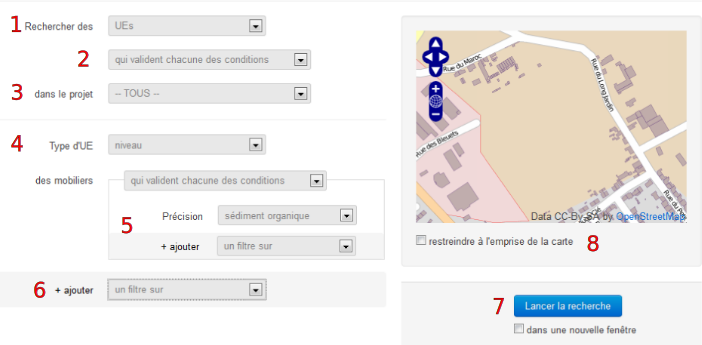
\includegraphics{recherche_ecran.png}}
\end{figure}


\subsection{Définir une cible}
\label{manuel/formulaire_recherche:definir-une-cible}
Pour effectuer une recherche, la première étape est de choisir le type de résultat à obtenir. Les résultats possibles couvrent l'ensemble des enregistrement qui peuvent être saisis dans l'application (UE, mobilier, matrice géologique, etc.).

Ce choix se fait dans la première liste du formulaire qui se nomme \emph{Rechercher des} (1).
\begin{figure}[htbp]
\centering

\scalebox{0.400000}{\includegraphics{recherche_cible_liste.png}}
\end{figure}


\subsection{Définir le périmètre de recherche}
\label{manuel/formulaire_recherche:definir-le-perimetre-de-recherche}
La seconde étape est de choisir dans une liste (3) si la recherche doit s'opérer sur un projet en particulier ou sur tous. Le premier choix permet de vous limiter à une seule source de réponses tandis que le second vous permet de faire des comparaisons entre les projets.

Le moteur vous propose ensuite de choisir entre les deux possibilités suivantes :
\begin{enumerate}
\item {} 
qui valident chacune des conditions : le résultat que vous obtiendrez répondra à tous les critères que vous mettrez en place, il suffit que l'enregistrement ne réponde pas positivement à un seul de ces critères pour qu'il ne fasse pas parti des résultats proposés.

\item {} 
qui valident une des conditions :  le résultat que vous obtiendrez répondra au moins à l'un des critères que vous mettrez en place.

\end{enumerate}

C'est à vous de définir si vous voulez des résultats répondant strictement à votre demande initiale ou si vous voulez un ensemble plus large de réponses pour éviter de passer à côté d'un résultat potentiellement intéressant.


\subsection{Définir les filtres}
\label{manuel/formulaire_recherche:definir-les-filtres}
Les filtres vont être le moyen d'obtenir uniquement les résultats qui concernent votre problématique, il s'agit d'utiliser les champs des différentes données stockées dans l'application pour limiter les résultats qui vous seront proposés.

Vous pouvez cumuler les filtres pour rajouter des conditions de tri, ce qui aura pour effet d'affiner les résultats qui vous seront soumis.

La première liste disponible vous propose d'ajouter un filtre sur l'un des attributs de votre cible (p. ex. \emph{Profil Paroi} si votre cible est l'UE) ou sur une relation.
\begin{figure}[htbp]
\centering

\scalebox{0.400000}{\includegraphics{recherche_filtre_liste.png}}
\end{figure}

L'ajout d'une relation permet d'ajouter des filtres sur les attributs d'un enregistrement lié à l'enregistrement cible.

\begin{notice}{note}{Note:}
\textbf{Exemple de recherche liée}

La possibilité de faire une recherche utilisant les relations permet d'être plus sélectif. Dans le cas d'une recherche de céramiques, en ajoutant un filtre sur le type d'UE \emph{fosse} et sur la phase \emph{occupation}, les résultats livrés par le moteur de recherche seront beaucoup plus réduits mais beaucoup plus probants.
\end{notice}

Il n'y a pas de limite au nombre de filtres que vous pouvez utiliser dans une recherche.

La carte présente sur cette page vous permet d'ajouter un type de filtre différent des autres. En cochant la case \emph{restreindre à l'emprise de la carte}, vous définissez une emprise spatiale pour votre recherche qui exclura toutes les données qui seront en dehors.


\subsection{Obtenir les résultats}
\label{manuel/formulaire_recherche:obtenir-les-resultats}
Une fois vos critères définis, vous pouvez obtenir la liste des résultats en cliquant sur le bouton \emph{Lancer la recherche}.

La case \emph{dans une nouvelle fenêtre} permet d'ouvrir la liste des résultats dans un nouvel onglet de votre navigateur, l'avantage de le faire est que vous pouvez revenir à tout moment sur la page de création de la recherche pour changer des paramètres et affiner vos critères.


\section{Utiliser les résultats}
\label{manuel/formulaire_recherche:recherche-utilisation}\label{manuel/formulaire_recherche:utiliser-les-resultats}\begin{figure}[htbp]
\centering

\scalebox{0.500000}{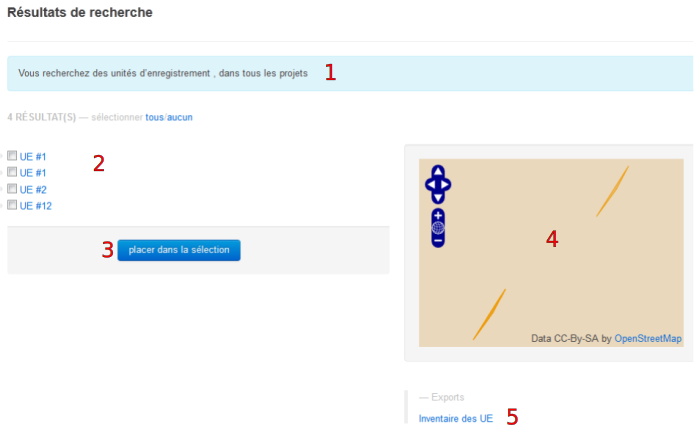
\includegraphics{recherche_resultat.png}}
\end{figure}

\textbf{1} Les critères de votre projet sont résumés en une phrase.

\textbf{2} Les résultats sont placés sous forme de liste, chaque résultat est précédé d'une case à cocher. La ligne d'en-tête de la liste se compose du total des résultats et des boutons \emph{tous} et \emph{aucun} qui vous permettent de cocher/décocher l'ensemble des résultats en un clic.

\textbf{3} Le bouton \emph{placer dans la sélection} permet de mettre tous les résultats dont les cases sont cochées dans votre panier de sélection. Cette fonction permet par exemple de rechercher les 8 fossés ayant livré du matériel lithique et de les assigner à la phase d'occupation du Néolithique.

\textbf{4} La carte va faire figurer tous les emplacements correspondant aux résultats, par exemple si vous recherchez des mobiliers céramiques vous obtiendrez sur cette carte les UE de provenance. Vous pouvez cliquer sur les formes géométriques pour sélectionner dans la liste le résultat correspondant.

\textbf{5} Le cadre \emph{Export} liste les différents classeurs que vous pouvez obtenir, ces exports se font au format CSV. Seuls sont exportés les résultats qui ont une case cochée.


\chapter{Questions fréquentes}
\label{manuel/questions_frequentes:questions-frequentes}\label{manuel/questions_frequentes::doc}

\section{Les formulaires}
\label{manuel/questions_frequentes:les-formulaires}

\subsection{Mon enregistrement a été modifié !}
\label{manuel/questions_frequentes:mon-enregistrement-a-ete-modifie}
Le SIA fonctionne en tant que serveur : à la différence d'un fichier Excel où le premier à l'ouvrir est le seul à pouvoir écrire, ici tous les utilisateurs peuvent lire et écrire en même temps. Si cela facilite grandement le travail en commun, cela signifie aussi que sur un formulaire de saisie \textbf{le dernier à cliquer} sur \emph{Enregistrer} sera celui dont l'enregistrement apparaîtra !

Pour éviter ce type de problèmes, il est conseillé de bien définir et répartir les rôles des utilisateurs d'un même projet. \textbf{La saisie des UE est à effectuer avant celle du mobilier}.


\subsection{Mon enregistrement a disparu !}
\label{manuel/questions_frequentes:def-valeurs-perdues}\label{manuel/questions_frequentes:mon-enregistrement-a-disparu}
Plusieurs raisons peuvent expliquer la disparition d'une fiche :
\begin{itemize}
\item {} 
\textbf{la suppression} : un utilisateur disposant des droits adéquats a cliqué sur \emph{supprimer}. La fiche n'est pas récupérable par un utilisateur. Si la perte est réellement importante (i.e. si elle n'est pas corrigeable manuellement en quelques minutes), les administrateurs disposent d'une copie journalière de la base données et peuvent restaurer les données perdues.

\end{itemize}

\begin{notice}{warning}{Warning:}
\textbf{Restaurer une fiche}

N'attendez pas trop longtemps avant de formuler une demande de restauration, les copies ne sont pas sauvegardées ad vitam !
Signalez quand votre projet est terminé afin de le clore et d'éviter ainsi des erreurs de manipulation (voir {\hyperref[manuel/formulaire_projet:projet-taches]{\emph{Répartition des tâches}}}).
\end{notice}
\begin{itemize}
\item {} 
\textbf{la dissociation} : certains enregistrements dépendent de leurs associations à une fiche parente pour être lié au projet, si cette association est sciemment rompue la fiche n'est alors plus accessible par les raccourcis habituels. Par exemple vous pouvez dissocier une mesure de son mobilier, de fait cette mesure devient orpheline. Pour restaurer la fiche, il faut faire une recherche sur \textbf{--AUCUN--} projet et sélectionner son type (mesure, document, etc.). La liste des résultats affichera alors toutes les fiches orphelines, vous pourrez alors en placer dans votre panier de sélection et restaurer l'association manuellement.

\item {} 
\textbf{l'écrasement} : l'UE 404 a disparu ? Un utilisateur a peut être tout simplement oublié d'ouvrir une fiche vierge et s'est simplement contenté d'effacer le numéro pour en mettre un nouveau.

\end{itemize}

\begin{notice}{warning}{Warning:}
\textbf{Créer une nouvelle fiche}

Ayez toujours le réflexe de passer par les raccourcis \emph{créer une nouvelle fiche xxxx}, vous éviterez ainsi d'écraser votre travail par inadvertance.
\end{notice}


\subsection{Les listes de valeurs et les champs ne me conviennent pas !}
\label{manuel/questions_frequentes:def-valeurs-manquantes}\label{manuel/questions_frequentes:les-listes-de-valeurs-et-les-champs-ne-me-conviennent-pas}
Les termes et les champs présents dans les différents formulaires ont deux principales origines :
\begin{itemize}
\item {} 
les arrêtés ministériels et préfectoraux relatifs à l'archéologie (p. ex. les normes d’inventaires documentaires et mobiliers), les termes et les champs sont alors figés et communs à tous les professionnels du monde archéologique.

\item {} 
les pratiques internes au CDA, les valeurs et les champs ont été recensés depuis les enregistrements terrain et post-fouille puis harmonisées afin d’éviter les redondances.

\end{itemize}

L’établissement d’un vocabulaire archéologique faisant consensus est une tâche ardue et que nul organisme n’a été en mesure de compiler, les termes utilisés par le CDA et utilisés par le SIA correspondent à la pratique opérationnelle et sont le produit de plusieurs dizaines d’opérations. De ce fait, ils recouvrent une bonne partie du vocabulaire spécifique aux opérations préventives.

Les listes du SIA sont figées, c'est-à-dire que chaque utilisateur emploie les mêmes termes que les autres sans possibilités de personnalisation. Cela permet d’assurer un enregistrement homogène dans tous les projets et d’éviter les écueils de thésaurus trop spécifiques et peu compréhensibles par le reste des usagers.

Des valeurs peuvent être ajoutées ou modifiées dans certaines listes après discussion entre les différents intervenants et validation. Toute modification est répercutée sur l’ensemble des projets, aussi bien ceux en cours que ceux archivés.


\subsection{La suppression de la fiche n'a pas supprimé ses relations !}
\label{manuel/questions_frequentes:la-suppression-de-la-fiche-n-a-pas-supprime-ses-relations}
La portée de la suppression est limitée à la fiche courante, par exemple la suppression d'un enregistrement de mobilier ne causera pas la perte de documents qui pourraient être utilisés par d'autres enregistrements. La suppression d'un enregistrement peut ainsi créer des orphelins (cas des mesures)


\section{Les exports}
\label{manuel/questions_frequentes:les-exports}

\subsection{Qu'est-ce qu'un fichier CSV ?}
\label{manuel/questions_frequentes:def-csv}\label{manuel/questions_frequentes:qu-est-ce-qu-un-fichier-csv}
\emph{Comma-separated values}, connu sous le sigle CSV, est un format informatique ouvert représentant des données tabulaires sous forme de valeurs séparées par des virgules. Un fichier CSV est un fichier texte, par opposition aux formats dits « binaires » tels que le XLS. Chaque ligne du texte correspond à une ligne du tableau et les virgules correspondent aux séparations entre les colonnes. Les portions de texte séparées par une virgule correspondent ainsi aux contenus des cellules du tableau.

Sous Excel, un simple double clic permet d'ouvrir le fichier avec un affichage en colonne. La plupart des logiciels capables de traiter des données tabulées gèrent l'importation de ce format (LibreOffice, Filemaker, 4D, etc.).


\subsection{A quoi correspond la colonne ``WKT'' ?}
\label{manuel/questions_frequentes:def-wkt}\label{manuel/questions_frequentes:a-quoi-correspond-la-colonne-wkt}
Le format Well-known text, abrégé en \emph{WKT}, peut se traduire par « texte bien lisible ». C'est un format standard en mode texte utilisé pour représenter des objets géométriques vectoriels issus des systèmes d’informations géographiques (SIG).

La présence de cette colonne vous permet d'importer le fichier CSV dans une application telle que Quantum GIS pour visualiser vos enregistrements de manière cartographique et dans le cas de l'export du mobilier, de produire des cartes de répartition en utilisant les données attributaires.


\subsection{Comment obtenir un export différent de ceux par défaut ?}
\label{manuel/questions_frequentes:comment-obtenir-un-export-different-de-ceux-par-defaut}
Pour des raisons de développement, ce nombre d'export est volontairement limité aux cas les plus courant, leur automatisation bénéficie à la plupart des utilisateurs. Si une exportation plus poussée mais non réalisable via le moteur de recherche vous est nécessaire, vous pouvez en faire la demande auprès des administrateurs qui essayeront de répondre à votre demande dans les limites du raisonnable.


\section{Le logiciel}
\label{manuel/questions_frequentes:le-logiciel}

\subsection{A qui appartient le SIA ?}
\label{manuel/questions_frequentes:a-qui-appartient-le-sia}
L'application-métier est la propriété du Centre départemental d'Archéologie du CG62.


\subsection{Quel est la licence utilisée ?}
\label{manuel/questions_frequentes:quel-est-la-licence-utilisee}
Tous les développements réalisés ont :
\begin{itemize}
\item {} 
soit la licence du logiciel utilisé lorsque celle-ci prime

\item {} 
soit la licence GPL dans le cas du code créé ex-nihilo

\end{itemize}


\subsection{Comment obtenir les sources ?}
\label{manuel/questions_frequentes:comment-obtenir-les-sources}
Bien qu'étant un logiciel libre, le code de l'application-métier n'est pour l'instant pas diffusé. Il a été décidé d'en éprouver le fonctionnement avant toute éventuelle mise à disposition externe.


\chapter{Équipe projet}
\label{manuel/participants::doc}\label{manuel/participants:equipe-projet}
Projet porté par le Centre départemental d’Archéologie, Conseil général du Pas-de-Calais


\section{Équipe Centre départemental d’Archéologie :}
\label{manuel/participants:equipe-centre-departemental-darcheologie}\begin{itemize}
\item {} 
Jean-Luc Marcy, directeur

\item {} 
Sophie François, chef du service des archives du sol

\item {} 
Jean-Roc Morreale, chargé du système d’informations archéologiques

\end{itemize}


\section{Équipe Direction des systèmes d’information :}
\label{manuel/participants:equipe-direction-des-systemes-dinformation}\begin{itemize}
\item {} 
Fabrice Douez, directeur

\item {} 
Laurent Bergamini, chef de projet

\item {} 
Olivier Watel, responsable de mission TIC - responsable Sécurité informatique

\item {} 
Philippe Beaucourt, chef de service Architecture et Expertise systèmes, réseaux, bases de données et Télécom

\end{itemize}


\section{Équipe Camptocamp :}
\label{manuel/participants:equipe-camptocamp}\begin{itemize}
\item {} 
Frédéric Jacon, chef de projet

\item {} 
Bruno Binet, ingénieur logiciel

\item {} 
Éric Lemoine, leader technique

\item {} 
Pierre Maudit, géomaticien développeur

\item {} 
François Van Der Biest, géomaticien, analyste développeur

\end{itemize}


\chapter{Lexique}
\label{manuel/lexique:lexique}\label{manuel/lexique::doc}\begin{itemize}
\item {} 
CDA : Centre Départemental d'Archéologie du Pas-de-Calais

\item {} 
Code entité : numéro attribué par le SRA, il peut découler d'une opération ou être distinct (ex. d'une entité issue d'une campagne de prospection)

\item {} 
Code opération : numéro d’opération archéologique attribué par le SRA

\item {} 
Collections : L’ensemble des vestiges mobiliers recueillis lors des opérations archéologiques et ou d’objets de provenances diverses regroupées par une même personne ou entité.

\item {} 
Diagnostic archéologique : Opération de terrain ayant pour but d’évaluer la densité, l’état de conservation et l’intérêt scientifique des vestiges archéologiques. Le diagnostic consiste en une opération généralement réalisée par le creusement de tranchées à la pelle mécanique sur 1/10ème de la surface qui sera aménagée.

\item {} 
DRAC : Direction Régionale des Affaires Culturelles

\item {} 
Fouille archéologique : Opération de terrain

\item {} 
Mobilier : Vestiges mobiliers recueillis lors des opérations archéologiques (céramique, verre, objets en métal, os, prélèvements, etc.)

\item {} 
PCR : Projet Collectif de Recherche

\item {} 
Projet non opérationnel : Les projets non opérationnels regroupent les autres projets. Exemple : projets de restauration, de conservation, de médiation, de valorisation et de prospection d’aménagement…

\item {} 
Projet opérationnel : Cette notion regroupe les opérations de terrain dont les fouilles et les diagnostics, c’est-à-dire les projets permettant de détecter et d’étudier les éléments du patrimoine archéologique susceptibles d’être affectés par ces travaux.

\item {} 
RO : Responsable d’Opération

\item {} 
SGBD : Système de Gestion de Base de Données

\item {} 
SIA : Système d'Informations Archéologiques

\item {} 
SIG : Système d’Information Géographique

\item {} 
SRA : Service Régional de l’Archéologie

\item {} 
UE : Unité d’Enregistrement

\item {} 
US : Unité Stratigraphique

\end{itemize}


\chapter{Liens}
\label{manuel/liens::doc}\label{manuel/liens:liens}

\section{SIA}
\label{manuel/liens:sia}\begin{itemize}
\item {} 
Geocatalogue \href{https://georchestra.archeologie.pasdecalais.fr/geonetwork/srv/fr/main.home}{https://georchestra.archeologie.pasdecalais.fr/geonetwork/}

\item {} 
Visualisateur \href{https://georchestra.archeologie.pasdecalais.fr/mapfishapp/}{https://georchestra.archeologie.pasdecalais.fr/mapfishapp/}

\end{itemize}


\section{Georchestra}
\label{manuel/liens:georchestra}\begin{itemize}
\item {} 
Site officiel de l'application \href{http://www.georchestra.org/}{http://www.georchestra.org}

\item {} 
Documentation utilisateur officielle \href{http://www.georchestra.org/documentation/index.html}{http://www.georchestra.org/documentation}

\end{itemize}


\section{Outils externes}
\label{manuel/liens:outils-externes}\begin{itemize}
\item {} 
Quantum GIS \href{http://www.qgis.org}{http://www.qgis.org}

\item {} 
Le Stratifiant \href{http://le-nid-du-stratifiant.ouvaton.org/}{le-nid-du-stratifiant.ouvaton.org}

\end{itemize}


\chapter{Indices and tables}
\label{index:indices-and-tables}


\renewcommand{\indexname}{Index}
\printindex
\end{document}
